%
% file: localoperator.tex
% author: Victor Brena
% description: Briefly describes properties of the local operator.
%

\chapter{Aromatic Amine Dehydrogenase}
\label{chap:aadh}

\section{Introduction}
\begin{figure}
    \centering
    \mycaption{Crystal Structure of aromatic amine dehydrogenase (AADH), PDB accession code: 2AGY \cite{masgrauAtomicDescriptionEnzyme2006}. The $\alpha$ sub-units are shown in green, the $\beta$ sub-units are in red, the Tryptophan Tryptophyl Quinone (TTQ) prosthetic group is shown as purple spheres.}
    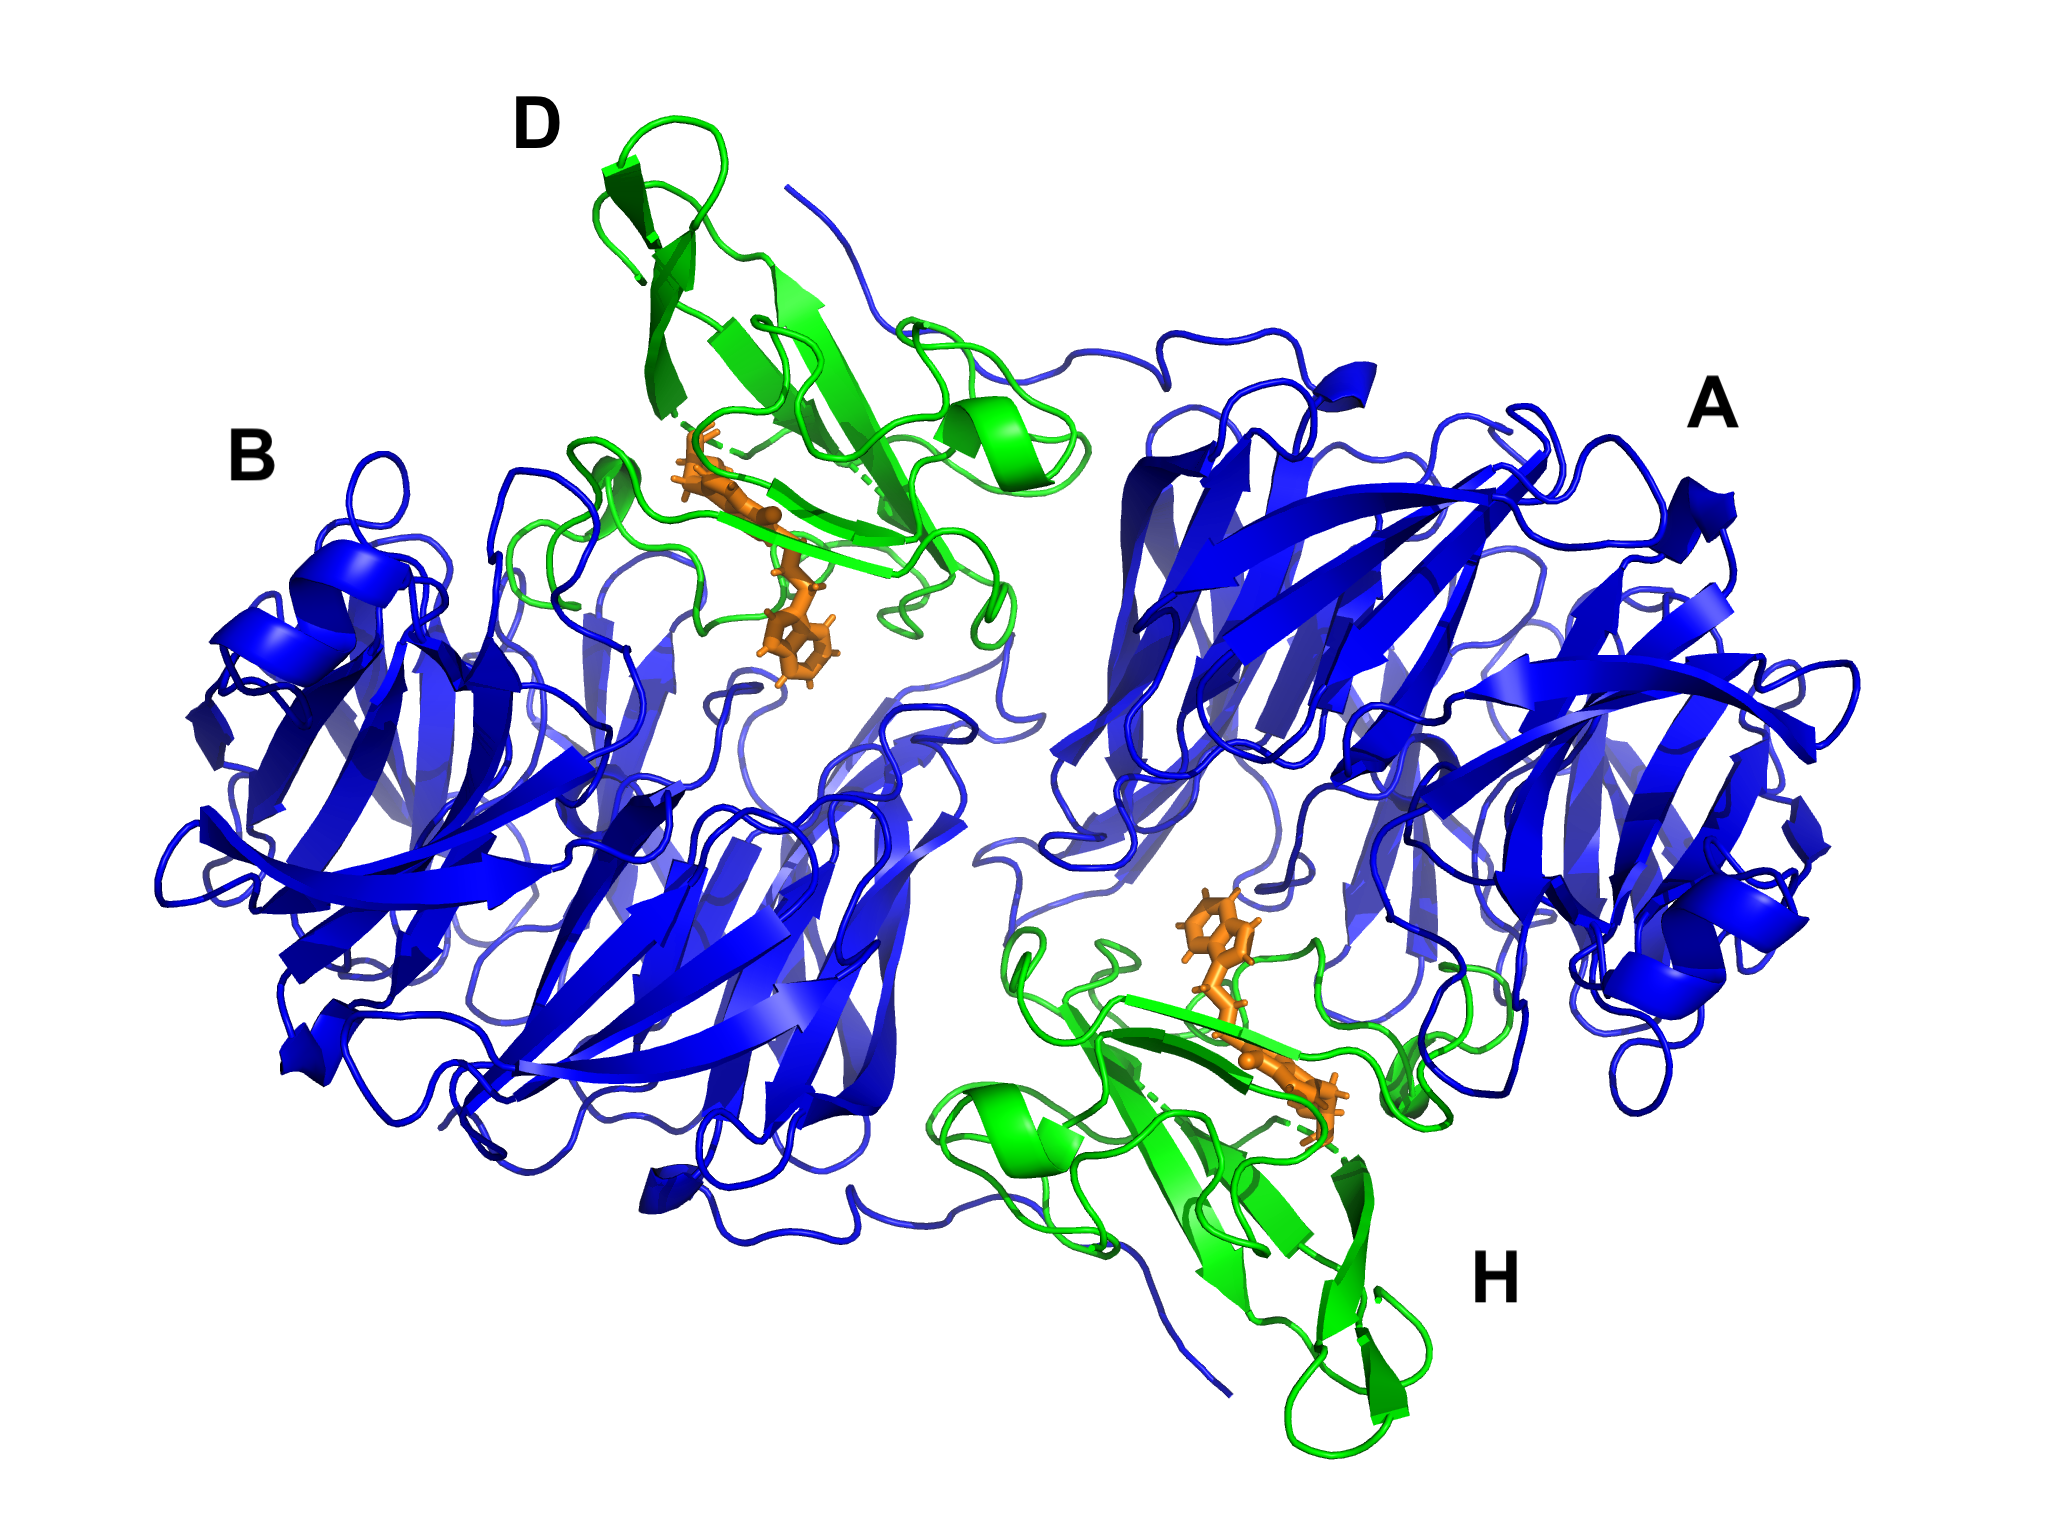
\includegraphics[width=0.8\textwidth]{chapters/aadh/figures/aadh_full_structure.png}
    \label{fig:aadh_full_structure}
\end{figure}

Aromatic Amine Dehydrogenase (AADH) is an enzyme of continued interest since its isolation and characterisation in 1983 \cite{iwakiCrystallizationPropertiesAromatic1983} because of its large kinetic isotope effect (KIE) \cite{hyunUnusuallyLargeIsotope1995a}\cite{basranImportanceBarrierShape2001a}  and the potential role of enzyme dynamics in its function \cite{mcgeaghProteinDynamicsEnzyme2011}\cite{glowackiProteinDynamicsEnzyme2012a}\cite{glowackiTakingOckhamRazor2012b}.  AADH oxidatively deaminates a range of different amines, but primarily aromatic amines \cite{hyunMechanisticStudiesAromatic1995a} to the corresponding aldehyde and ammonia using a covalently bound Tryptophan tryptophylquinone (TTQ) prosthetic group \cite{govindarajAromaticAmineDehydrogenase1994a}. The protein has an $\alpha_{2}\beta_{2}$ structure shown in figure \ref{fig:aadh_full_structure}. The larger $\alpha$ sub-units have a mass of $\simeq \SI{39}{\kilo\dalton}$ (shown in green) while the smaller $\beta$ sub-units (shown in red) have a mass of $\simeq \SI{18}{\kilo\dalton}$. The $\beta$ sub-units contain the TTQ prosthetic group that forms part of the active site (shown in purple spheres, after reaction with tryptamine). 


\begin{figure}[p]
    \centering
    \mycaption{The proposed reaction mechanism of AADH, adapted from figure 2 in \cite{masgrauAtomicDescriptionEnzyme2006}. The TTQ prosthetic group is shown in purple, the Asp128$\beta$ group in red and the tryptamine substrate in blue. The boxed step $4$ is the rate determining tunnelling step and step $7$ is the oxidation step. }
    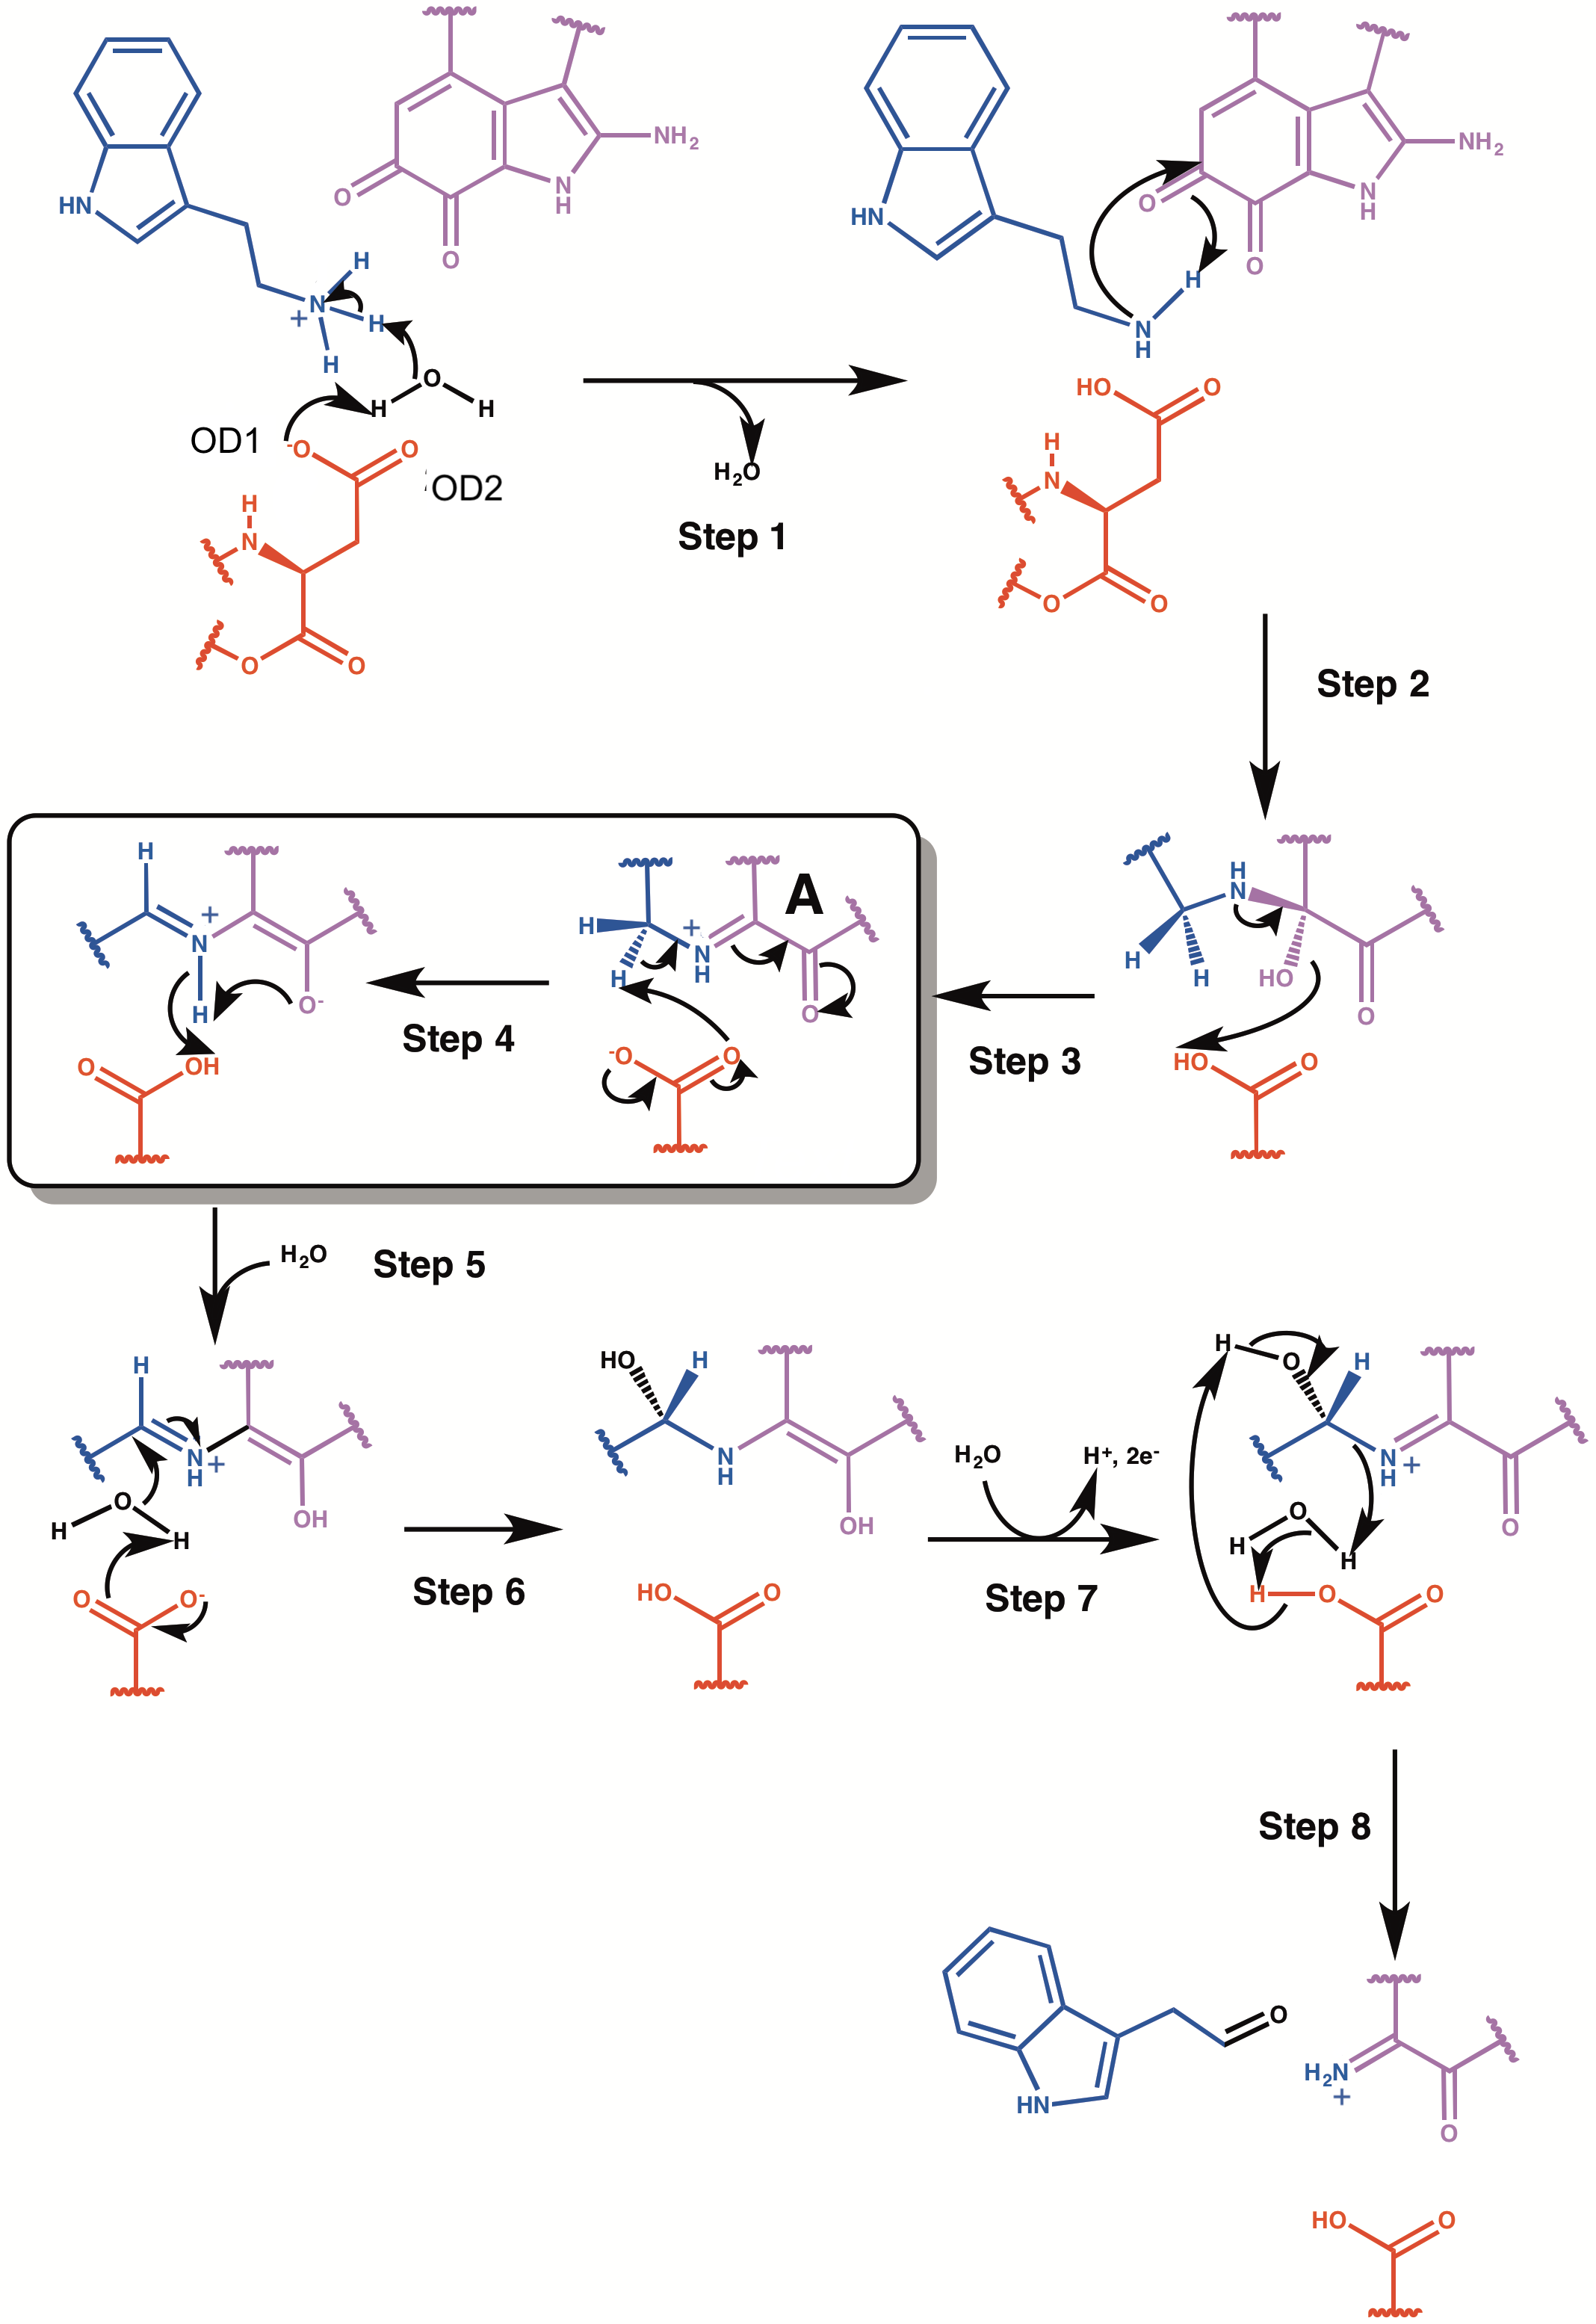
\includegraphics[width=0.8\textwidth]{chapters/aadh/figures/aadh_mechanism.png}
    \label{fig:aadh_mechanism}
\end{figure}

The reaction mechanism of AADH was proposed in \cite{hyunMechanisticStudiesAromatic1995a} and more fully elucidated by a combination x-ray crystallography, experimental and QM/MM (with increasing levels of theory) in \cite{masgrauAtomicDescriptionEnzyme2006}\cite{masgrauTunnelingClassicalPaths2007} and \cite{ranaghanInitioQMMM2017} using tryptamine as a substrate. 
The reaction mechanism is shown in figure \ref{fig:aadh_mechanism}, adapted from figure 2 in \cite{masgrauAtomicDescriptionEnzyme2006}.  The TTQ prosthetic group, attached to the $\beta$ sub-unit, is shown in purple, the protonated tryptamine substrate is shown in blue and the Asp128 residue is shown in red.  The mechanism starts with the enzyme substrate complex of the protonated tryptamine situated next to the TTQ group and Asp128 residue.  The tryptamine is deprotonated by oxygen 1 of the Asp128 residue via a bridging water molecule (step 1).  The nitrogen atom on the tryptamine attacks one of the carbonyl groups of the TTQ residue to form a carbinol-amine intermediate (step 2) that then goes on to form the iminoquinone intermediate labelled `A' (step 3).  Intermediate A was not observed directly but was inferred from the crystal structure of an analogous complex using phenylhydrazine in place of tryptamine.  Step 4, shown boxed, is the rate determining step and involves the tunnelling of a proton from the tryptamine carbon atom adjacent to the nitrogen, to an oxygen atom of the Asp128 residue.  The proton is shown here accepted by oxygen 2 of the Asp128 carboxylate group, but in principle oxygen 1 could also serve as an acceptor. The oxyanion on the TTQ/substrate group (hereafter referred to as TTW) is then neutralized by protonation from Asp128 via the hydrogen atom on the protonated Schiff base (step 5). Water is introduced and in step 6 attacks the Schiff base to form a carbinolamine intermediate that is then oxidized in step 7.  The carbinolamine is then hydrolysed in step 8 and releases the aldehyde.  


The experimental free energy barrier for this reaction is $\simeq \SI{12.7}{\kilo\cal\per\mol}$ at $T=\SI{300}{\kelvin}$ with a primary kinetic isotope effect of $55 \pm 6$, independent of temperature for $T =$ \SIrange{278}{298}{\kelvin}\cite{masgrauAtomicDescriptionEnzyme2006}. The high KIE is indicative of the hydrogen tunneling through the reaction barrier  \cite{masgrauAtomicDescriptionEnzyme2006}\cite{kohenEnzymeCatalysisClassical1998}\cite{antoniouInternalEnzymeMotions2001}\cite{antoniouLargeKineticIsotope1997}\cite{allemannQuantumTunnellingEnzymecatalysed2009}. The rate determining hydrogen abstraction can proceed to either OD1 or OD2 of the Asp128. These two atoms are distinguished by the hydrogen bonded network: OD2 is hydrogen bonded to Trp160, and OD1 to Thr172 as shown in figure \ref{fig:aadh_active_site}. In the previous AADH simulation studies,  \cite{masgrauAtomicDescriptionEnzyme2006}\cite{masgrauTunnelingClassicalPaths2007}\cite{ranaghanInitioQMMM2017}, the authors labelled OD1 as O2 and OD2 as O1, this convention is not adopted here as the accessible conformations allow OD1 and OD2 to bond to both Trp160 and Thr172, the force-field atoms names will be retained. 

The authors of \cite{ranaghanInitioQMMM2017} calculated the potential energy surface for pathways to both oxygen atoms using nudged elastic band with QM/MM using DH\&HLYP/6-311+G(d)/MM. Although not the aim of this study, they incorporated zero-point energy, tunneling and entropic contributions of previous studies \cite{masgrauAtomicDescriptionEnzyme2006}\cite{masgrauTunnelingClassicalPaths2007} to estimate the free energy barriers to O2 and O1 as $\SI{11.5}{\kilo\cal\per\mol}$ and $\SI{8.84}{\kilo\cal\per\mol}$ respectively, meaning both pathways are distinct but indistinguishable from the experimental free energy.  

The role of protein dynamics in promoting tunneling has proved controversial in part due to the problems with identifying the contribution of the enzyme over a suitable reference reaction [][][]. However, current theory \cite{kuznetsovProtonHydrogenAtom1999a}\cite{masgrau2004hydrogen} uses two types of protein dynamics to explain the rate constants and the temperature dependence of the KIE. `Active dynamics' which enhance the probability of tunneling occurring in a given conformation, and `passive dynamics' which re-arrange the enzyme to achieve such a suitable conformation. Active vibrations, on the sub-picosecond timescale,  have been identified in AADH \cite{johannissenEnzymeAromaticAmine2008}\cite{johannissenProtonTunnelingAromatic2007} which act to promote the tunneling reaction.  However, the KIE in AADH is independent of temperature \cite{masgrauAtomicDescriptionEnzyme2006}, indicative of passive dynamics being the dominant factor in explaining the observed rate constant. Furthermore in  \cite{glowackiProteinDynamicsEnzyme2012a}\cite{glowackiTakingOckhamRazor2012b} the authors showed that the kinetics and KIEs of a number of enzymes with large KIEs, including AADH, could be fitted to a simple extension of Transition State Theory (TST). This model posits two inter-converting enzyme conformations each linked to a reaction coordinate with different reaction barriers. While this model can be made to  realistically fit experimental data, the conformers, their number and the exact values of the model parameters have not been fully validated. 

It is clear that an accurate and comprehensive description of the conformational dynamics of AADH would be useful in adding to the ongoing debate of enzyme dynamics and their role in catalysis. This chapter describes the first step towards this goal, the creation of molecular dynamics data set and the estimation of important parameters of the system for use in later chapters. The structure is as follows: section \ref{sec:aadh_md} describes the creation of a molecular dynamics data set; section \ref{sec:aadh_validation} validates the data set, in particular active sites and compares to previous work; section \ref{sec:aadh_msm} describes the creation of a Markov State Model in order to estimate the Markov lag time and the number of dominant eigenvalues which will be used in the optimisation of MSM hyper-parameters in chapters \ref{chap:msm} and \ref{chap:hmm}. 

\section{Molecular dynamics}\label{sec:aadh_md}

The starting point was crystal structure of AADH in Schiff base form after reaction with tryptamine, PDB accession code 2AGY \cite{masgrauAtomicDescriptionEnzyme2006}. Dr Kara Ranaghan prepared the PDB file by adding the missing hydrogen atoms, determining the protonation states of titratable residues, created the disulphide bridges and parameterized the TTQ/Tryptamine Schiff base (structure A in figure \ref{fig:aadh_mechanism}, custom residue name TTW) for use with the CHARMM-22 forcefield \cite{a.d.mackerellAllAtomEmpiricalPotential1998} as part of the computational part of \cite{masgrauAtomicDescriptionEnzyme2006}, \cite{masgrauTunnelingClassicalPaths2007} and \cite{ranaghanInitioQMMM2017}.  The first 23 residues of the D and H segments, which were unobserved in the crystal structure, were not modelled. This concludes Dr Ranaghan's contribution to this work. 

The atom types in TTW were changed to be compatible with the CHARMM-36 \cite{huangCHARMM36AllatomAdditive2013} force-field although the TTW parameters remained the same. The CHARMM package, version 42a2 \cite{brooksCHARMMBiomolecularSimulation2009} was used to create a protein structure file (PSF). 

A solvation shell tracking the surface of the protein was created using the package Solvate version 1.0 \cite{grubmullerSolvate} which I modified to take into account the CHARMM extended PSF format. The shell was $\SI{12.0}{\angstrom}$ thick, the maximum boundary curvature radius of the solvent surface was $\SI{100}{\angstrom}$, and $10$ Gaussian functions were used to determine the solvent surface. This structure was further solvated to create a cubic simulation cell of size $\SI{130}{\angstrom}$ using the package Visual Molecular Dynamics (VMD) version 1.9.3 \cite{HUMP96} with a boundary parameter equal to $\SI{1.2}{\angstrom}$. The size of the box was chosen so that the minimum distance between the enzyme and the edge of the simulation cell was  $\SI{14}{\angstrom}$. The system was neutralized with VMD using sodium chloride to attain a concentration of $\SI{0.15}{\molar}$. 
The minimization, heating and equilibration steps were performed in CHARMM with the OpenMM \cite{OpenMMRapidDevelopment} plug-in using the CHARMM-36m \cite{huangCHARMM36AllatomAdditive2013} force-field. The electronic non-bonded forces in all steps were treated with partial mesh Ewald summation with a cut-off of $\SI{14}{\angstrom}$, all other parameters were set to their default values. The SHAKE \cite{ryckaertNumericalIntegrationCartesian1977b} algorithm was used throughout to constrain the hydrogen atoms. The minimization proceeded by first constraining all heavy atoms  using a Root Mean Square Deviation (RMSD) constraint with a mass weighted force constant of $\SI{5}{\kilo\cal\per\mol\per\angstrom}$ and then minimizing with $100$ step using the steepest descent algorithm and $3000$ steps of Adopted Basis Newton-Raphson (ABNR) minimization. This was repeated and sequentially limiting the  constraint to the heavy protein atoms, heavy protein backbone atoms, and finally with no constraints. The final unconstrained minimization proceeded with $5000$ instead of $3000$ ABNR minimization. 

The system was heated from $\SI{10}{\kelvin}$ to $\SI{310}{\kelvin}$ in steps of $\SI{25}{\kelvin}$ with a harmonic constraint on the heavy protein backbone atoms with mass weighted force constant of $\SI{5}{\kilo\cal\per\mol\per\angstrom}$ and . At each heating step $\SI{10}{\pico\second}$ of Langevin dynamics in a constant volume, constant temperature ensemble were run with a time-step of $\SI{2}{\femto\second}$ and collision frequency of $\gamma=\SI{5}{\per\pico\second}$. 

The system underwent equilibration in two stages: constrained equilibration and unconstrained equilibration. In the restrained equilibration stage $11 \times \SI{20}{\pico\second}$ iterations of Langevin dynamics were run in an constant pressure, constant temperature ensemble ($P=\SI{1}{\atm}$, $T=\SI{310}{\kelvin}$), with a Langevin collision frequency $\gamma=\SI{1}{\per\pico\second}$, a Monte Carlo barostat with volume moves performed every  $\SI{50}{\femto\second}$, and a time-step of $\SI{2}{\femto\second}$. On the first iteration the backbone atoms had a harmonic constraint with a mass weighted force constant of  $\SI{10}{\kilo\cal\per\mol\per\angstrom}$. On each subsequent iteration the force constant was reduced by $\SI{1}{\kilo\cal\per\mol\per\angstrom}$ until the last iteration had no harmonic constraint. The unconstrained equilibration consisted of $\SI{200}{\pico\second}$ of equilibration was run under the same conditions as before with no constraints. 

The simulation system was transferred to AMBER 16 \cite{caseAMBER} and a single  $\SI{100}{\nano\second}$ trajectory was produced in a constant volume, constant temperature ($T=\SI{310}{\kelvin}$) ensemble, using Langevin dynamics with a collision frequency of $\gamma=\SI{5}{\per\pico\second}$, and a time step of $\SI{2}{\femto\second}$. The non-bonded cut-off distance was reduced to $\SI{12}{\angstrom}$ and SHAKE was used to constrain the hydrogen atoms. Coordinates and velocities were written to disk every $\SI{100}{\pico\second}$.  

The coordinates and velocities at every \SIlist[list-final-separator = { ... }]{1; 2; 100}{\nano\second} were used to seed $100 \times \SI{100}{\nano\second}$ new trajectories, run under the same conditions. These $100$ trajectories constituted the AADH data set. 

\section{Validation}\label{sec:aadh_validation}

An error was found in the preparation of the initial structure \emph{after} completion of the simulations. The disulphide bridge between Cys81 and Cys113 on the H segment (but not on the D segment) had not been created, instead the two thiol groups were left unoxidized. This will be discussed in full below. 

\begin{figure}
    \centering
    \mycaption{Structural similarity of trajectory used to seed the the final production trajectories. Panel (a) shows the $\alpha$-Carbon RMSD relative to the crystal structure, (b) shows the distribution of all pairwise $\alpha$-Carbon RMSD.   }
    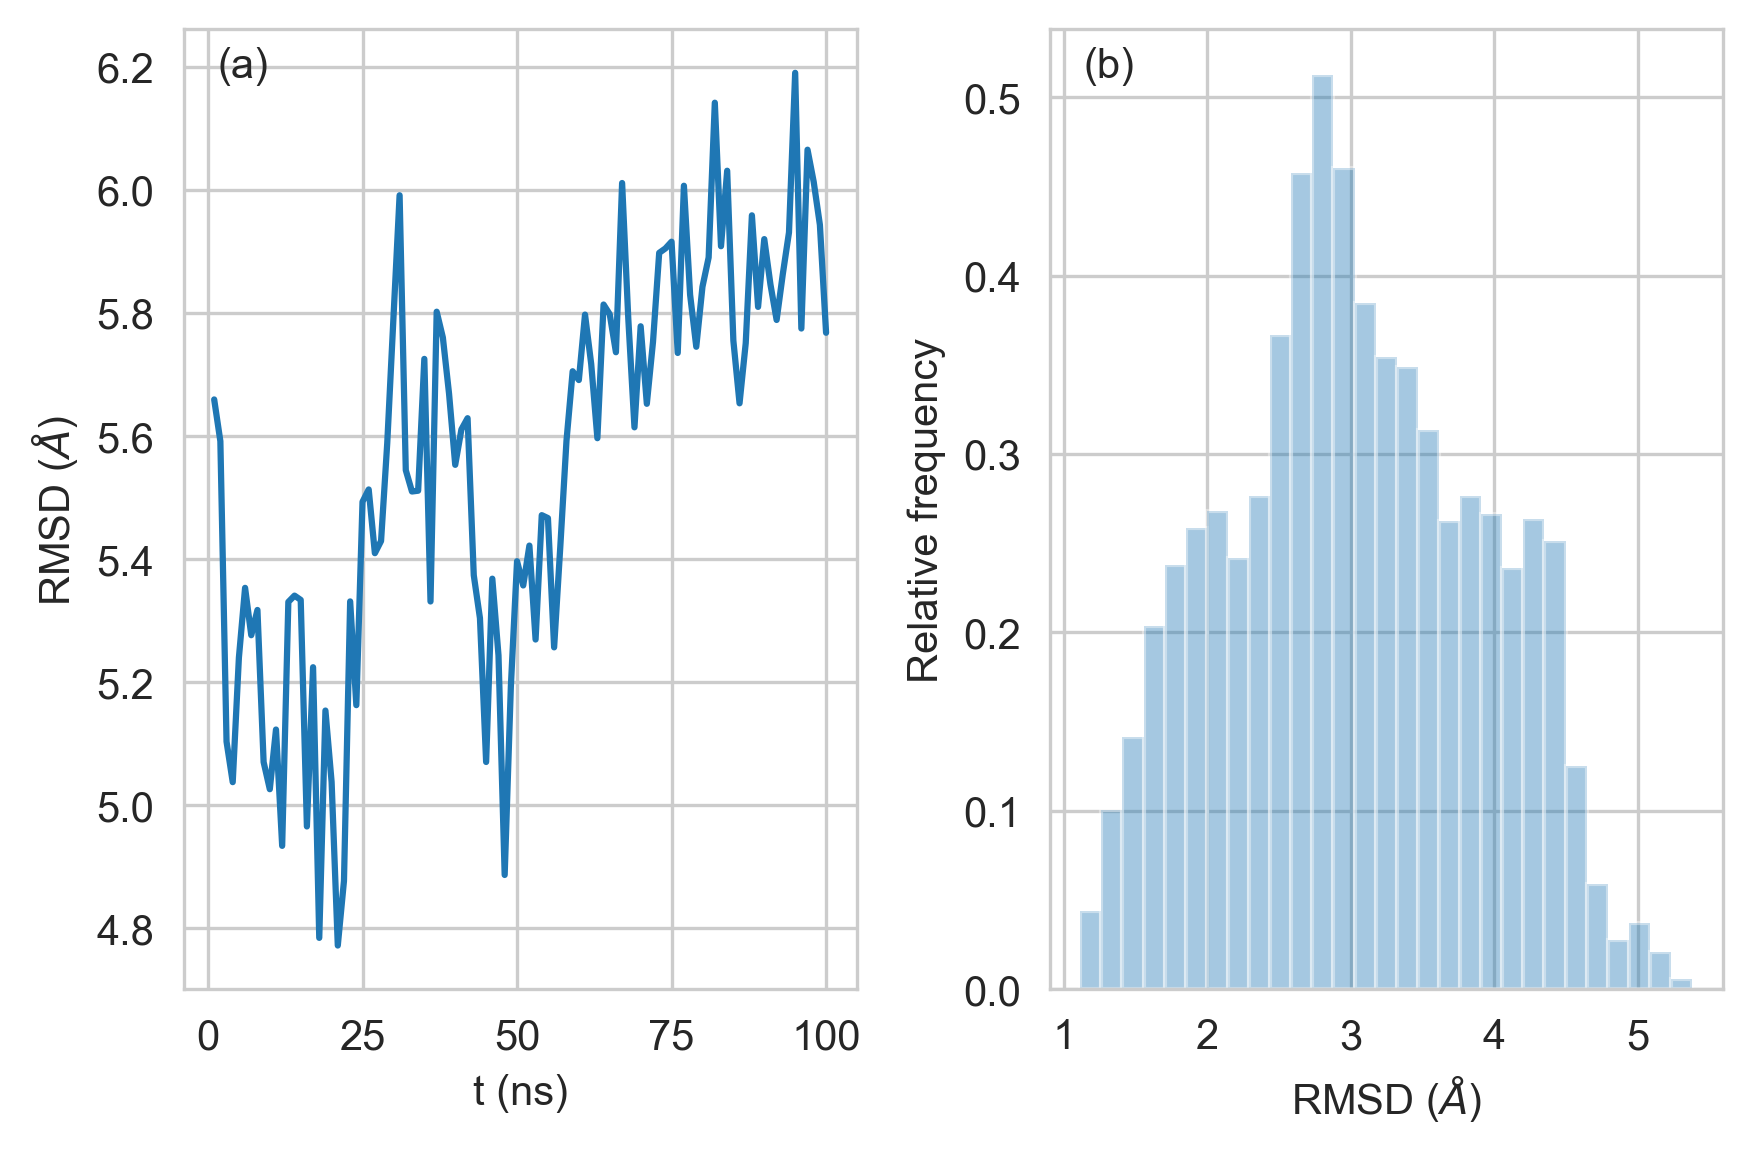
\includegraphics[width=0.8\textwidth]{chapters/aadh/figures/rmsd_seed_trajectory.png}
    \label{fig:rmsd_seed_traj}
\end{figure}

 The structural similarity between these initial frames of the $100$ trajectories is shown in figure \ref{fig:rmsd_ca}. Panel (a)  shows the $\alpha$-Carbon RMSD, relative to the crystal structure, of the initial frames. This clearly shows serial correlation between initial frames, especially for those at $t>\SI{60}{\nano\second}$. Panel (b) shows the distribution of $\alpha$-Carbon RMSD values between each pair of initial frames (so there are $\sfrac{1}{2}\cdot 100\cdot 99$ values) which demonstrate a range of differences between the initial conformations. $\SI{50}{\percent}$ of the initial structures have an RMSD of $\SI{3.0}{\angstrom}$ or larger.  

Each trajectory was checked for structural stability over the course of the simulations by calculating the RMSD of the $\alpha$-Carbons atoms relative to the crystal structure. The majority of the trajectories showed no breakdown in structure, with  \SI{95}{\percent} of the frames within \SIrange{4.5}{6.4}{\angstrom} of the crystal structure. However, seven of the trajectories ($24, 27, 30, 42, 78, 87$ and $97$) had an RMSD trajectory which increased over time, leaving the upper \SI{95}{\percent} bound by at least the final frame, shown in figure \ref{fig:rmsd_ca}. To check that these trajectories weren't losing their secondary structure the number of residues in each simplified secondary structure class \cite{kabschDictionaryProteinSecondary1983} over time were calculated. Each trajectory showed a stable number of residues in each class as shown in figure \ref{fig:dssp_trajs}.

\begin{figure}
    \centering
    \mycaption{The crystal structure of the active site of AADH. This definition is taken from \cite{ranaghanInitioQMMM2017}. The yellow dashed lines show the important stabilizing hydrogen bonds as well as the H/O distances involved in the rate determining step.  The reactive hydrogen atoms are labelled HI-2 and HI-3. The acceptor oxygen atoms are labelled O1 (OD2) and O2 (OD1). All other hydrogen atoms are hidden.}
    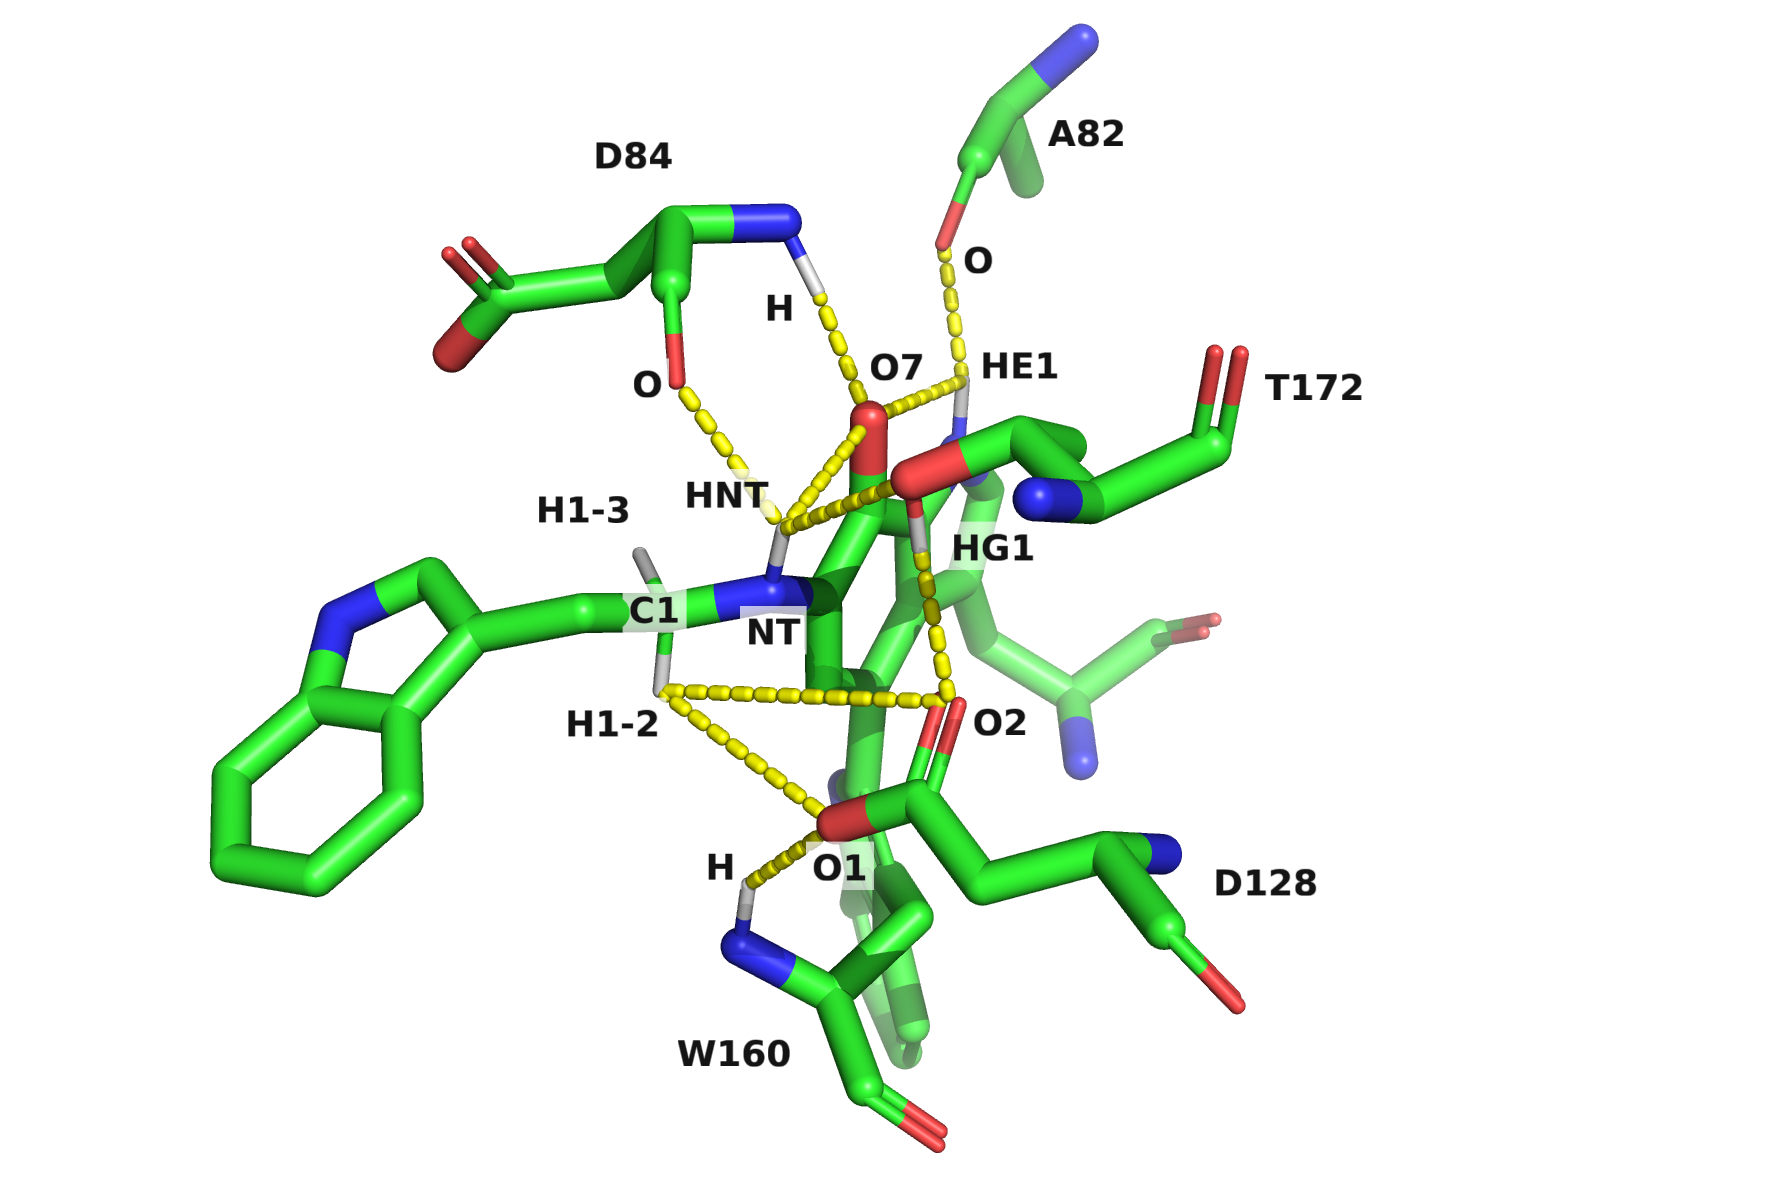
\includegraphics[width=0.8\textwidth]{chapters/aadh/figures/aadh_active_site.png}
    \label{fig:aadh_active_site}
\end{figure}

\begin{figure}
    \centering
    \mycaption{The distribution of heavy atom RMSD, relative to the crystal structure of the active sites in segment D (blue) and H (orange). }
    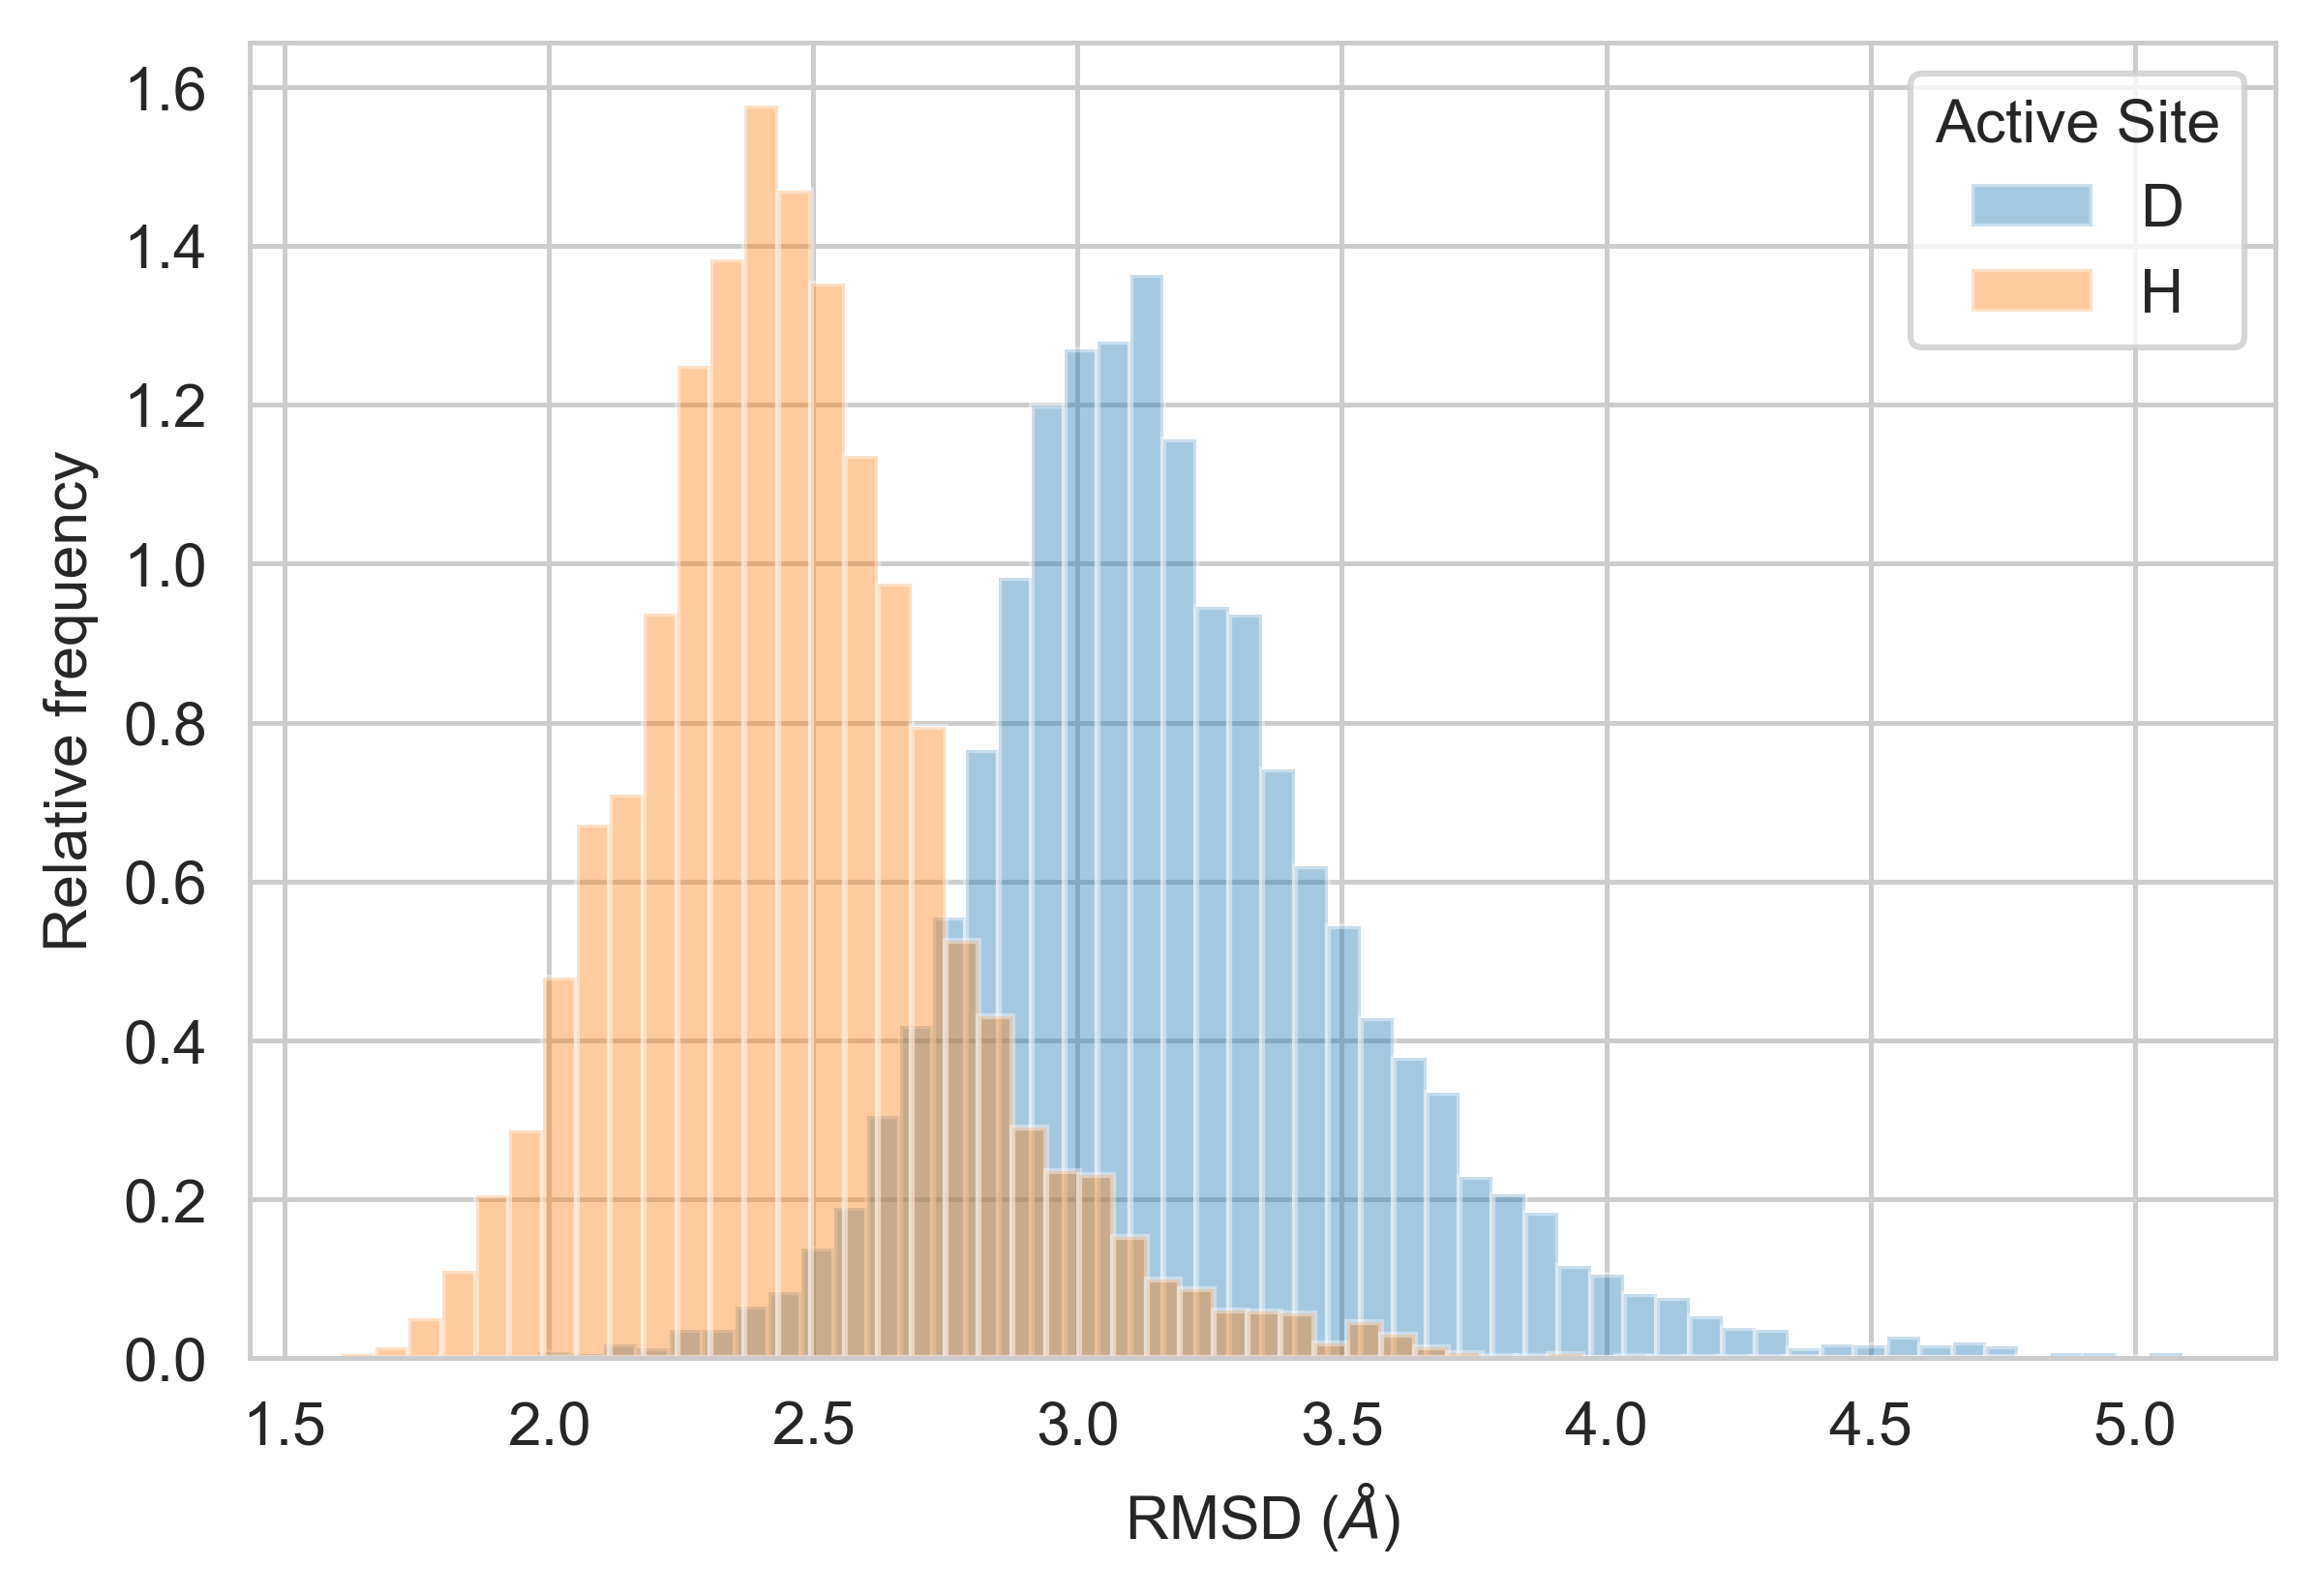
\includegraphics{chapters/aadh/figures/rmsd_dististribution.png}
    \label{fig:as_rmsd_dist}
\end{figure}

The active site of the enzyme was defined (following \cite{ranaghanInitioQMMM2017}, \cite{masgrauAtomicDescriptionEnzyme2006} and \cite{masgrauTunnelingClassicalPaths2007}) as the following residues in both segments D and H: Ala82, Asp84, TTW109, Asp128, Trp160 and Thr172. The TTW residue is the TTQ prosthetic group after reaction with the tryptamine substrate to form the Schiff base intermediate. Any references to TTQ will refer to the potion of TTW coming from TTQ originally and not the unreacted prosthetic group. The crystal structure of the active site is shown in figure \ref{fig:aadh_active_site}. 

The structures of the two active sites were compared to the crystal structure. The distribution of the heavy atom RMSD, relative to the crystal structure, is shown in figure \ref{fig:as_rmsd_dist}. This shows that, surprisingly, the H active site, without the di-sulphide bridge is more structurally similar to the crystal structure than the D active site. 

\begin{figure}
    \centering
    \mycaption{Distribution of bond distances in the active site. Panels (a) - (d) show the four combinations of acceptor ion (O1, O2) - proton (H1-2, H1-3) distances; panels (e) and (f) are the two donor (C1) acceptor (O1, O2) distances; the remaining panels are the hydrogen bonds in the active site.}
    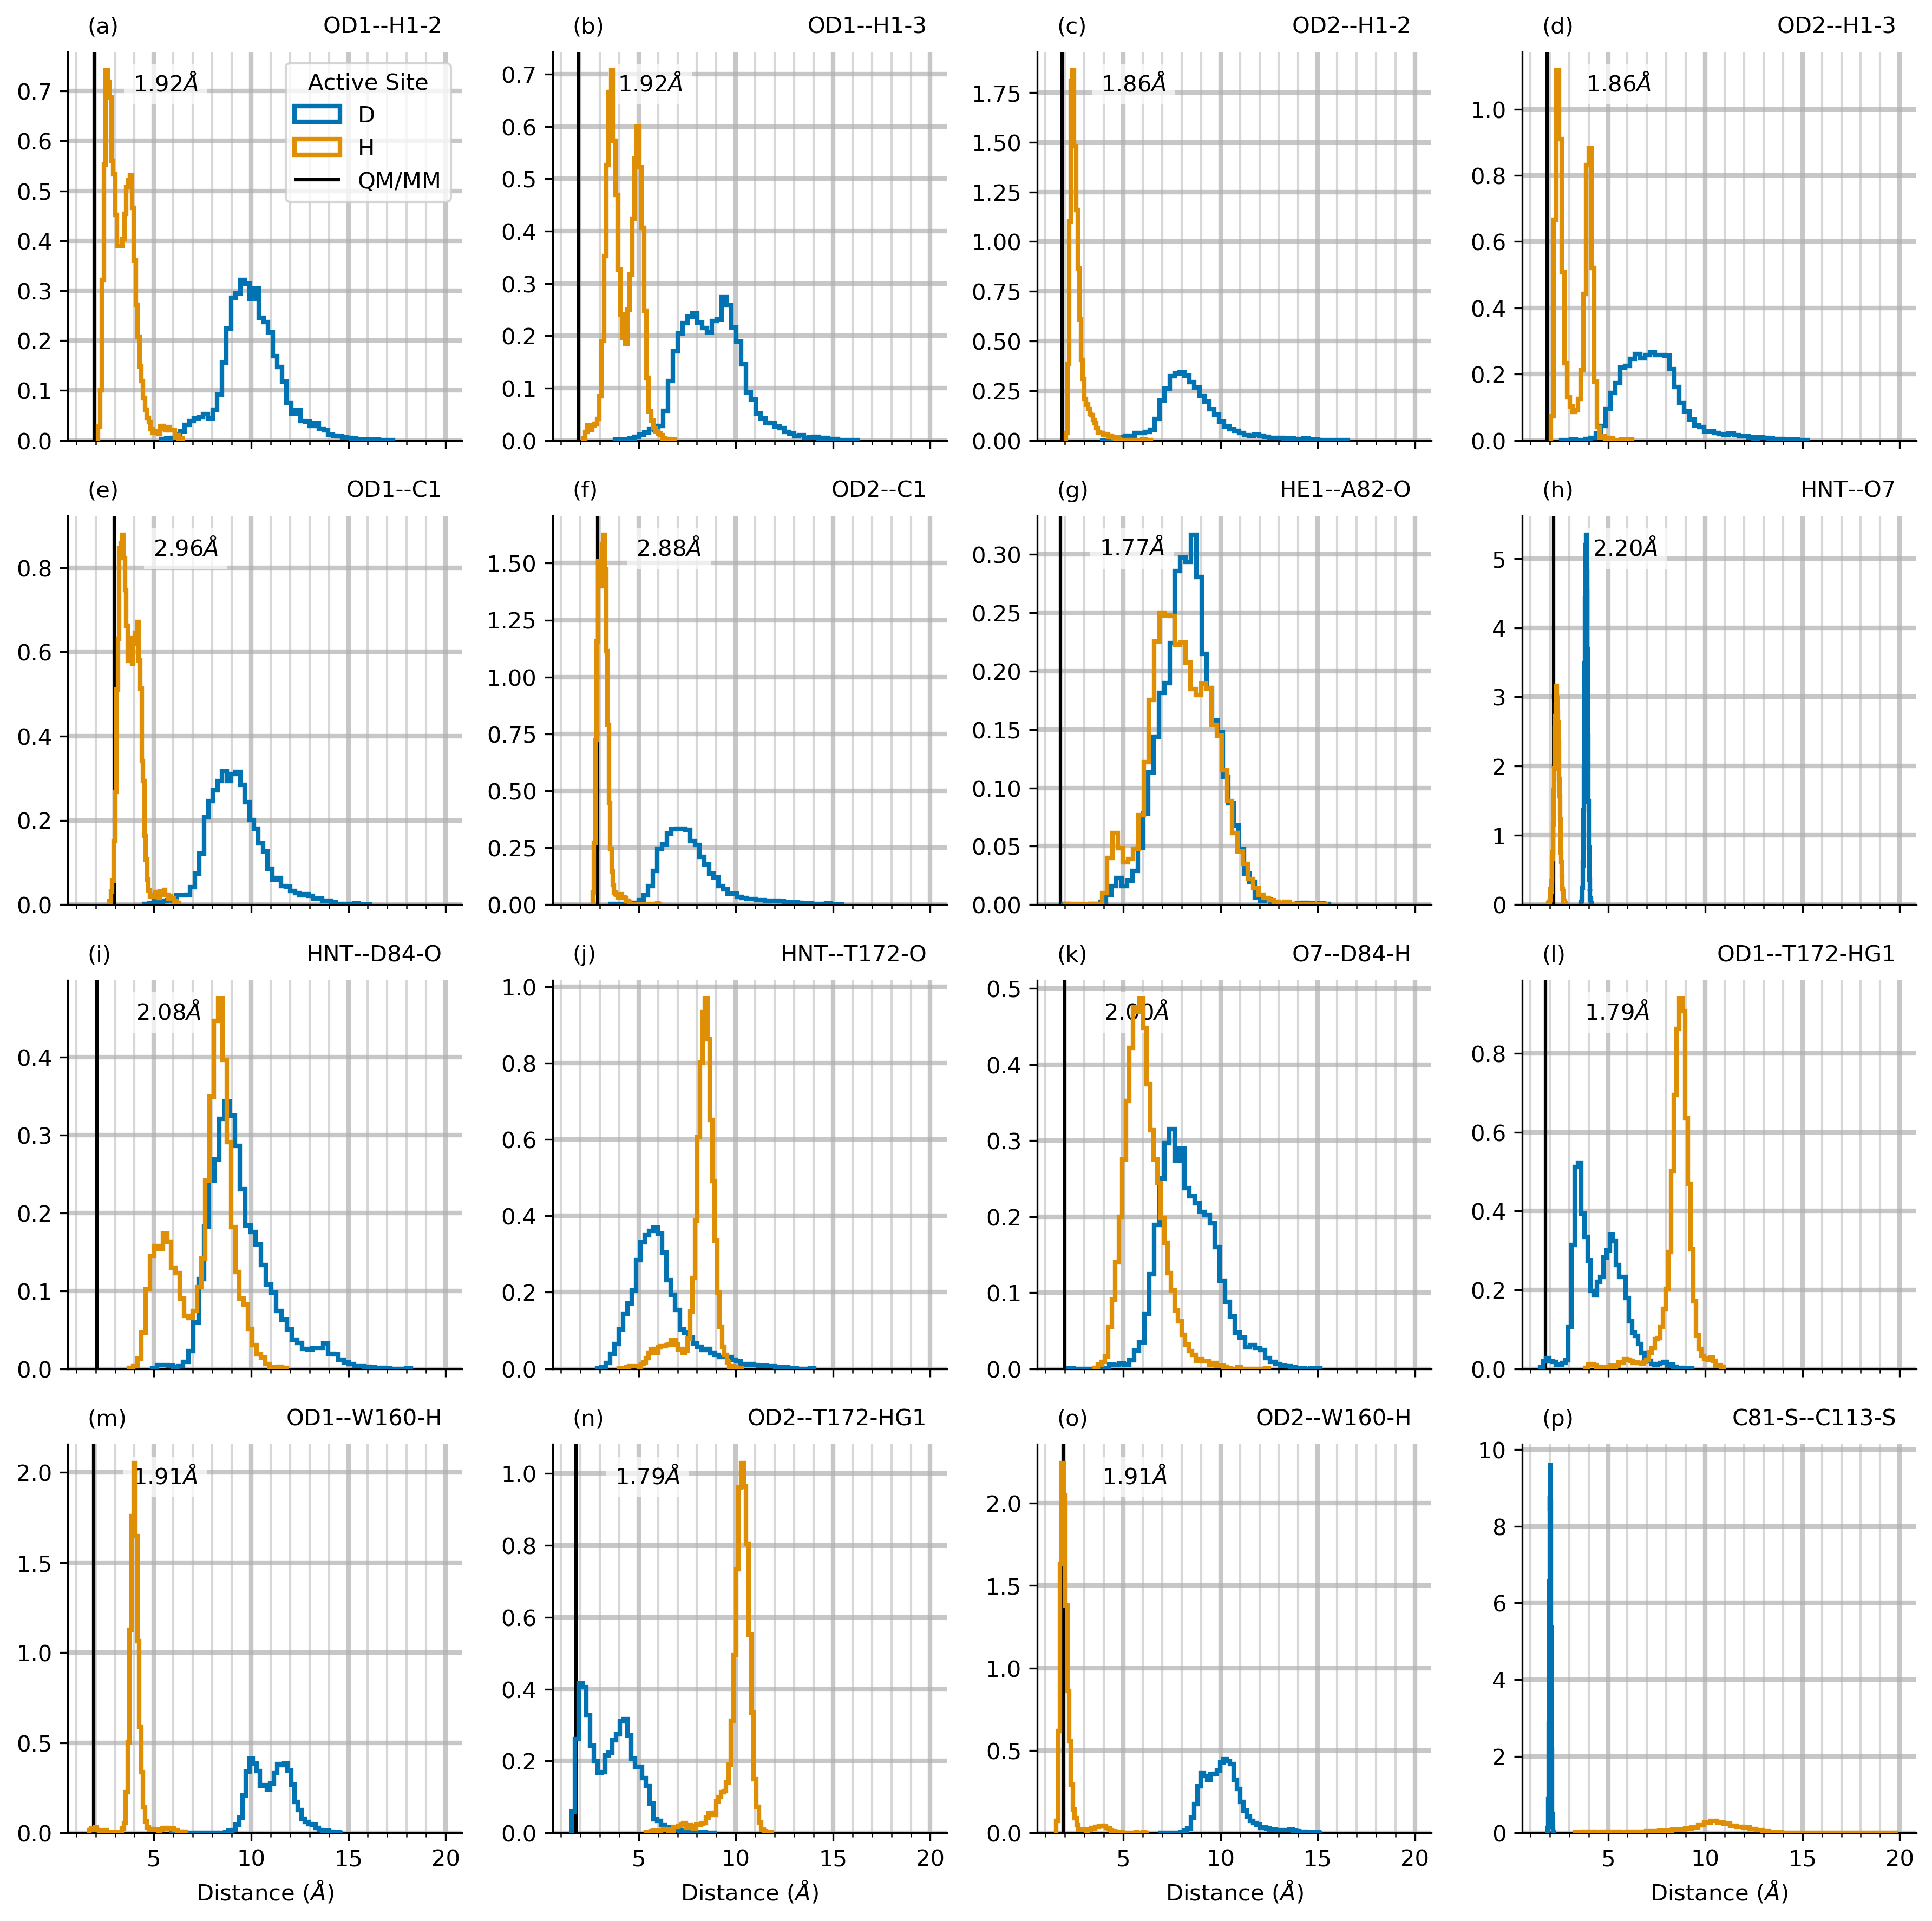
\includegraphics[width=0.8\textwidth]{chapters/aadh/figures/bond_distances_dist.png}
    \label{fig:bond_dist}
\end{figure}

To understand this difference between the active sites further and to explore the similarities between these simulations and the most accurate previous work in \cite{ranaghanInitioQMMM2017}, the distribution of important interatomic distances were calculated and compared. Figure \ref{fig:bond_dist} shows these bond distributions in blue for the D active site and in orange for the H active site. The black vertical lines with labels are the QM/MM interatomic distances in the reactant state\footnote{An average over the pathways to OD1 and OD2 are taken where appropriate.}, taken from table 3 of \cite{ranaghanInitioQMMM2017}. Where possible I have kept the atom labels the same as \cite{ranaghanInitioQMMM2017}, the exceptions are the atoms directly involved in bond breaking and formation. The correspondence between the interatomic distances in \cite{ranaghanInitioQMMM2017} and figure \ref{fig:bond_dist}, and their description are as follows: 
\begin{enumerate}
    \item O1/O2---H1:  The bond being formed. These correspond to all four combinations of distances between OD2/OD1 (respectively) and H1-2, H1-3. Shown in panels (a) through (d). 
    \item O1/O2---C1: The donor/acceptor distance. These are the two combinations of distances between OD2/OD1 (respectively) and C1. Shown in panels (e) and (f). 
    \item HE1---O7: Intra-residue hydrogen bond in the TTQ prosthetic group shown in panel (g). This bond distance is effectively fixed by the molecular mechanics force-field. \label{he1_07}
    \item HE1---A82-O: Inter-residue hydrogen bond between HE1 of the TTQ prosthetic group and the Ala82 backbone oxygen atom, shown in panel (h). 
    \item HNT---O7: Intra-residue hydrogen bond in the TTW residue. Shown in panel (i). 
    \item HNT---D84-O: Inter-residue hydrogen bond between the TTW residue and the backbone oxygen atom of the Asp84 residue. 
    \item HNT---T172-O: This is not described in \cite{ranaghanInitioQMMM2017} but is included because of its potential to form a hydrogen bond in certain conformations. Shown in panel (k). 
    \item O7---D84-H: Inter-residue hydrogen bond between the TTW residue and the backbone amide hydrogen atom of the Asp84 residue. Shown in panel (l). 
    \item O2---T172-HG1/W160-H: The inter-residue hydrogen bond between the acceptor oxygen atom OD1 of D128 and hydrogen atoms on the Thr172 and Trp160 residues respectively. Shown in panels (m) and (n).
    \item O1---T172-HG1/W160-H: The inter-residue hydrogen bond between the acceptor oxygen atom OD2 of D128 and hydrogen atoms on the Thr172 and Trp160 residues respectively. Shown in panels (o) and (p).\label{o1_t172}
    \item C81-S---C113-S: The di-sulphide bond in the D and H segments.\label{cs_cs} 
\end{enumerate}

The missing di-sulphide bond has clearly had a large effect on H active site. The distribution of the S---S distances in the H active site, shown in panel (q) varies between  \SIrange{3}{20}{\angstrom} compared to the effectively fixed distance of $\simeq \SI{2}{\angstrom}$ in the D active site. The distributions in the D active site show greater variance and do not, in general, overlap with those in the H active site. 

The O---H distances are smaller, closer to the QM/MM values, and show less variation in the H active site compared to the D active site by a significant margin (panels (a) - (d)). The distances in the H site are almost all less than \SI{5}{\angstrom} (within $\simeq\SI{3}{\angstrom}$ of the QM/MM values), where almost all the D active site values are between \SIrange{5}{10}{\angstrom}. The donor/acceptor distances, C---O (panels (e) and (f)) show a similar story. The closest hydrogen atom to both acceptor oxygen anions in the H active site is H1-2, the differences in the D active site are less obvious.

There is no conclusive similarity between the QM/MM results and these simulations with respect to the hydrogen bond network stabilizing OD1 and OD2 by Thr172 and Trp160. The orientation of Trp160-H, OD2, OD1 and Thr172-HG1 in the crystal structure and QM/MM is approximately linear. For OD1 to be hydrogen bonded with Thr172, the bond lengths would be ordered OD1---Thr172-HG1 $<$ OD1-Trp160-H, i.e. panel (m) $<$ panel (n). While for OD2 to be hydrogen bonded with Trp160, the bond lengths would be ordered OD2---Thr172-HG1 $>$ OD2-Trp160-H, i.e. panel (o) $>$ panel (p). This is clearly the case for the H active site. In the D active site, Asp128 has moved away from Trp160 entirely as seen by comparing the distributions in  panels (n) and (p)  with panels (m) and (o). Noting that TTW is covalently bonded to Trp160, this is then consistent with the picture in panels (a) through (f) where OD1 and OD2 are between \SIrange{5}{15}{\angstrom} from the relevant atoms on TTW.  

The intra-residue hydrogen bonds in TTW involving O7, show good agreement with the QM/MM values. HE1---O7 (panel (g)) is almost fixed by the rigid tryptophan ring system and is the same in both H and D active sites. The HNT---O7 distance in the H active site is in agreement with QM/MM while the D active site it larger by almost \SI{2}{\angstrom}. The two distinct HNT---O7 bond lengths define whether the NT---C1 bond is either syn or anti the C---O7 carbonyl bond in the tryptophan ring system of TTQ. The anti conformation, with has the shorter HNT---O7 distance, is adopted in active site H and in the crystal structure as shown in figure \ref{fig:aadh_active_site}.  Here the NT---HNT bond points in the same direction as the C---O7 bond and forcing the NT---C1 bond into the anti-conformation. The syn conformation has the has the NT---HNT bond pointing in the opposite direction, forcing the NT---C1 bond to eclipse the the C---O7 carbonyl bond. 

The syn and anti conformations allow radically different conformational states to be accessed as demonstrated in figure \ref{fig:ttw_wiggle}. Each panel shows $500$ conformational states, selected evenly across all trajectories, for the D (panel (a)) and H (panel (b)) active site. The entire TTW residue and carbonyl group of Asp128 is shown and the conformations have been aligned to the tryptophan part of the TTW residue. The only two hydrogen atoms shown are H1-2 \& H1-3 and are coloured white. The syn conformation of the D active site clearly demonstrates a `looser' set of conformations with the  C1-H1 bond pointing away from the acceptor Asp128 residue. The anti conformation of the H active site shows a `tighter' set of conformations with the C1-H1 bond pointing towards the Asp128 residue. 


\begin{figure}
    \centering
    \mycaption{Conformations of the TTW residue in the D and H active sites. Five conformations were taken from each trajectory at intervals of $\SI{20}{\nano\second}$ and aligned along the heavy atoms of the trypotophan part of the TTQ residue.  The hydrogen atom shown is the donor atom, all other hydrogen atoms are hidden.}
    \subbottom[Active site D]{
    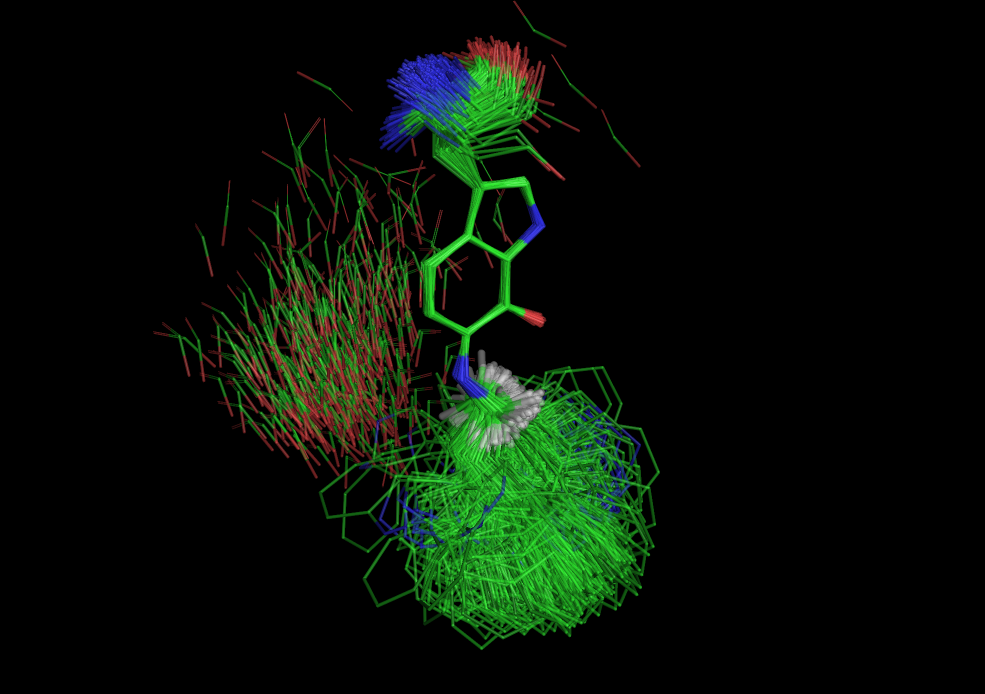
\includegraphics[trim={1cm, 0, 1cm, 0}, clip=True]{chapters/aadh/figures/as_d_wiggle.png}}
    \subbottom[Active site H]{
    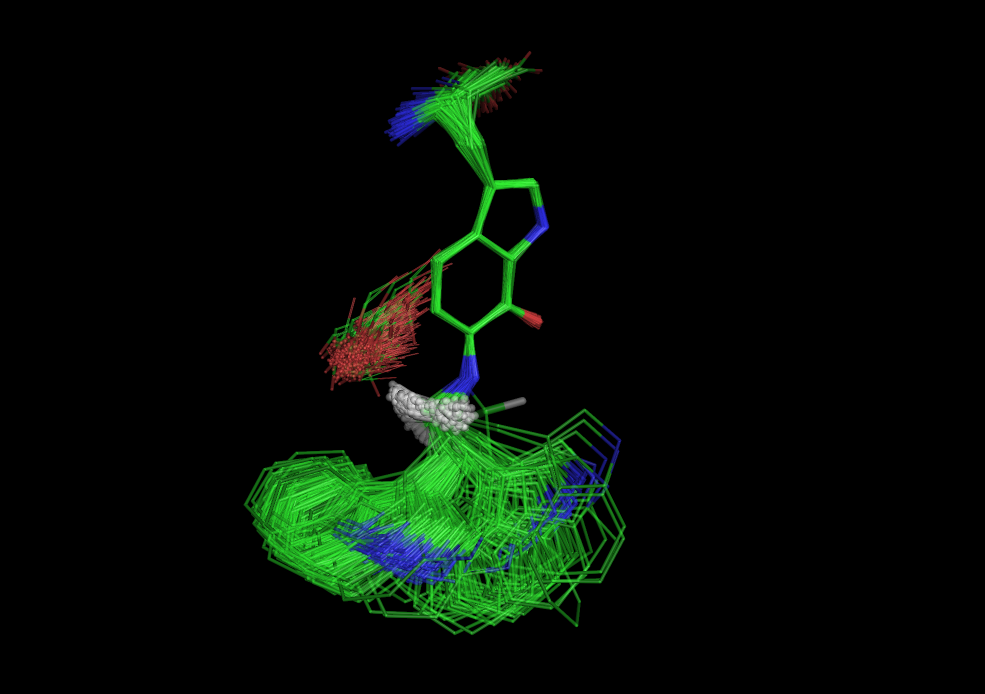
\includegraphics[trim={1cm, 0, 1cm, 0}, clip=True]{chapters/aadh/figures/as_h_wiggle.png}
    }
    \label{fig:ttw_wiggle}
\end{figure}

In summary, the two active sites show distinct differences in the accessible conformations due to the missing di-sulphide bridge between residues Cys81 and Cys113. The two sites are differentiated in three main ways. First, the relevant interatomic distances and hydrogen bonds between TTW and Asp128 in the H but not in the D active site, are consistent with the QM/MM results. Second, the orientation of the NT-C1 bond is syn the C---O7 carbonyl bond in the D active site, whereas in the H active site and QM/MM results, it is anti. Third, the H site is more constrained with less variation in the available conformations compared to the  D active site. These apparent compatibility of the H active site with QM/MM results are surprising given the missing di-sulphide bridge occurs in the H active site. Despite this, only the  coordinate trajectories for the D active site will be used in all further analysis.  

\section{Estimating $\tau$ and $k$}\label{sec:aadh_msm}

The conformational dynamics and metastable states of the active site of AADH will be explored later chapters. In particular, chapter \ref{chap:msm} will detail the how to choose the trajectory pre-processing choices (hyper-parameters) to estimate an optimal MSM. This requires fitting and evaluating a number of MSMs which in turn requires the specification of a Markov lag time ($\tau(\mathrm{MSM})$) and the number, $k$, dominant eigenvalues. 

In order to estimate these two values for AADH the eigenvalue and implied timescale spectra, resulting from a single set of pre-processing choices, were investigate. The following results are for the D active site only, given the error in the H active site simulation. A similar analysis, albeit with different conclusions, was originally performed for the H site, these are not described. 

The trajectories were discretized by first projecting the cartesian coordinates onto a set of features, applying TICA to reduce the dimension of the feature space and then clustering the frames into a small set of discrete states.  The features used were the bond lengths identified in \cite{ranaghanInitioQMMM2017} i.e. those whose histograms are depicted in panels (a) - (f), (h), (j), (l), (m), (p) of figure \ref{fig:bond_dist}. The intra-molecular hydrogen bonds in panels (g) and (i) were excluded due to their small variance. The trajectories were sub-sampled resulting in a time step of $\SI{0.1}{\nano\second}$. TICA was applied with a lag time of $\tau=\SI{1}{\nano\second}$ and the number of components retained set so as to retain $\SI{95}{\percent}$ of the variance which equated to $m=10$ components retained. The k-means clustering was used to cluster the trajectories into $n=\lfloor\sqrt{N}\rfloor = 316$ discrete states. This was based on the heuristic described in \cite{husicWardClusteringImproves2017a} where $N$ is the number of MD frames.  

The Markov lag time must be chosen large enough so that the Markov assumption holds. This equates to the implied timescales ($t_{i}=-\sfrac{\tau(\mathrm{MSM})}{\ln{|\lambda_{i}|}}$) being independent of $\tau(\mathrm{MSM})$. However, the eigenvalue spectrum will be heavily influenced by choice of hyper-parameters, in particular the protein feature. So a suitable lag time for this particular set of hyper-parameters may not prove suitable for another set. In other words, a suitable lag time cannot be chosen independent of the hyper-parameters, but the hyper-parameters cannot be optimised without specifying a lag time. The same reasoning also applies to the number of dominant eigenvalues, except that the number of dominant processes determines the number of eigenvalues used in the VAMP-2 score. 

\begin{figure}
    \centering
    \mycaption{The implied timescales and relative VAMP-2 scores as a function of the Markov lag time $\tau(\mathrm{MSM})$. Panel (a) shows the first five implied timescales for $\SI{0}{\nano\second} < \tau(\mathrm{MSM}) < \SI{5}{\nano\second}$, panel (b) shows the first five implied timescales for $\SI{0}{\nano\second} < \tau(\mathrm{MSM}) < \SI{50}{\nano\second}$. The solid lines and coloured shaded areas are the mean and \SI{95}{\percent} credible intervals respectively, estimated using MCMC with $500$ posterior samples. The grey shaded area is the region for which the implied timescales are smaller than the lag time. Panel (c) and (d) show the VAMP-2 scores, scored on the first $2-5$ eigenvalues for the same ranges. The VAMP-2 scores are indexed to $1$ at their initial value. The colour coding is consistent between the implied timescale plots and VAMP-2 plots. So that $k=2$, in blue, is the score including the first eigenvalue $\lambda = 1$ and the eigenvalue of the longest implied timescale also shown in blue in panels (a) and (b). }
    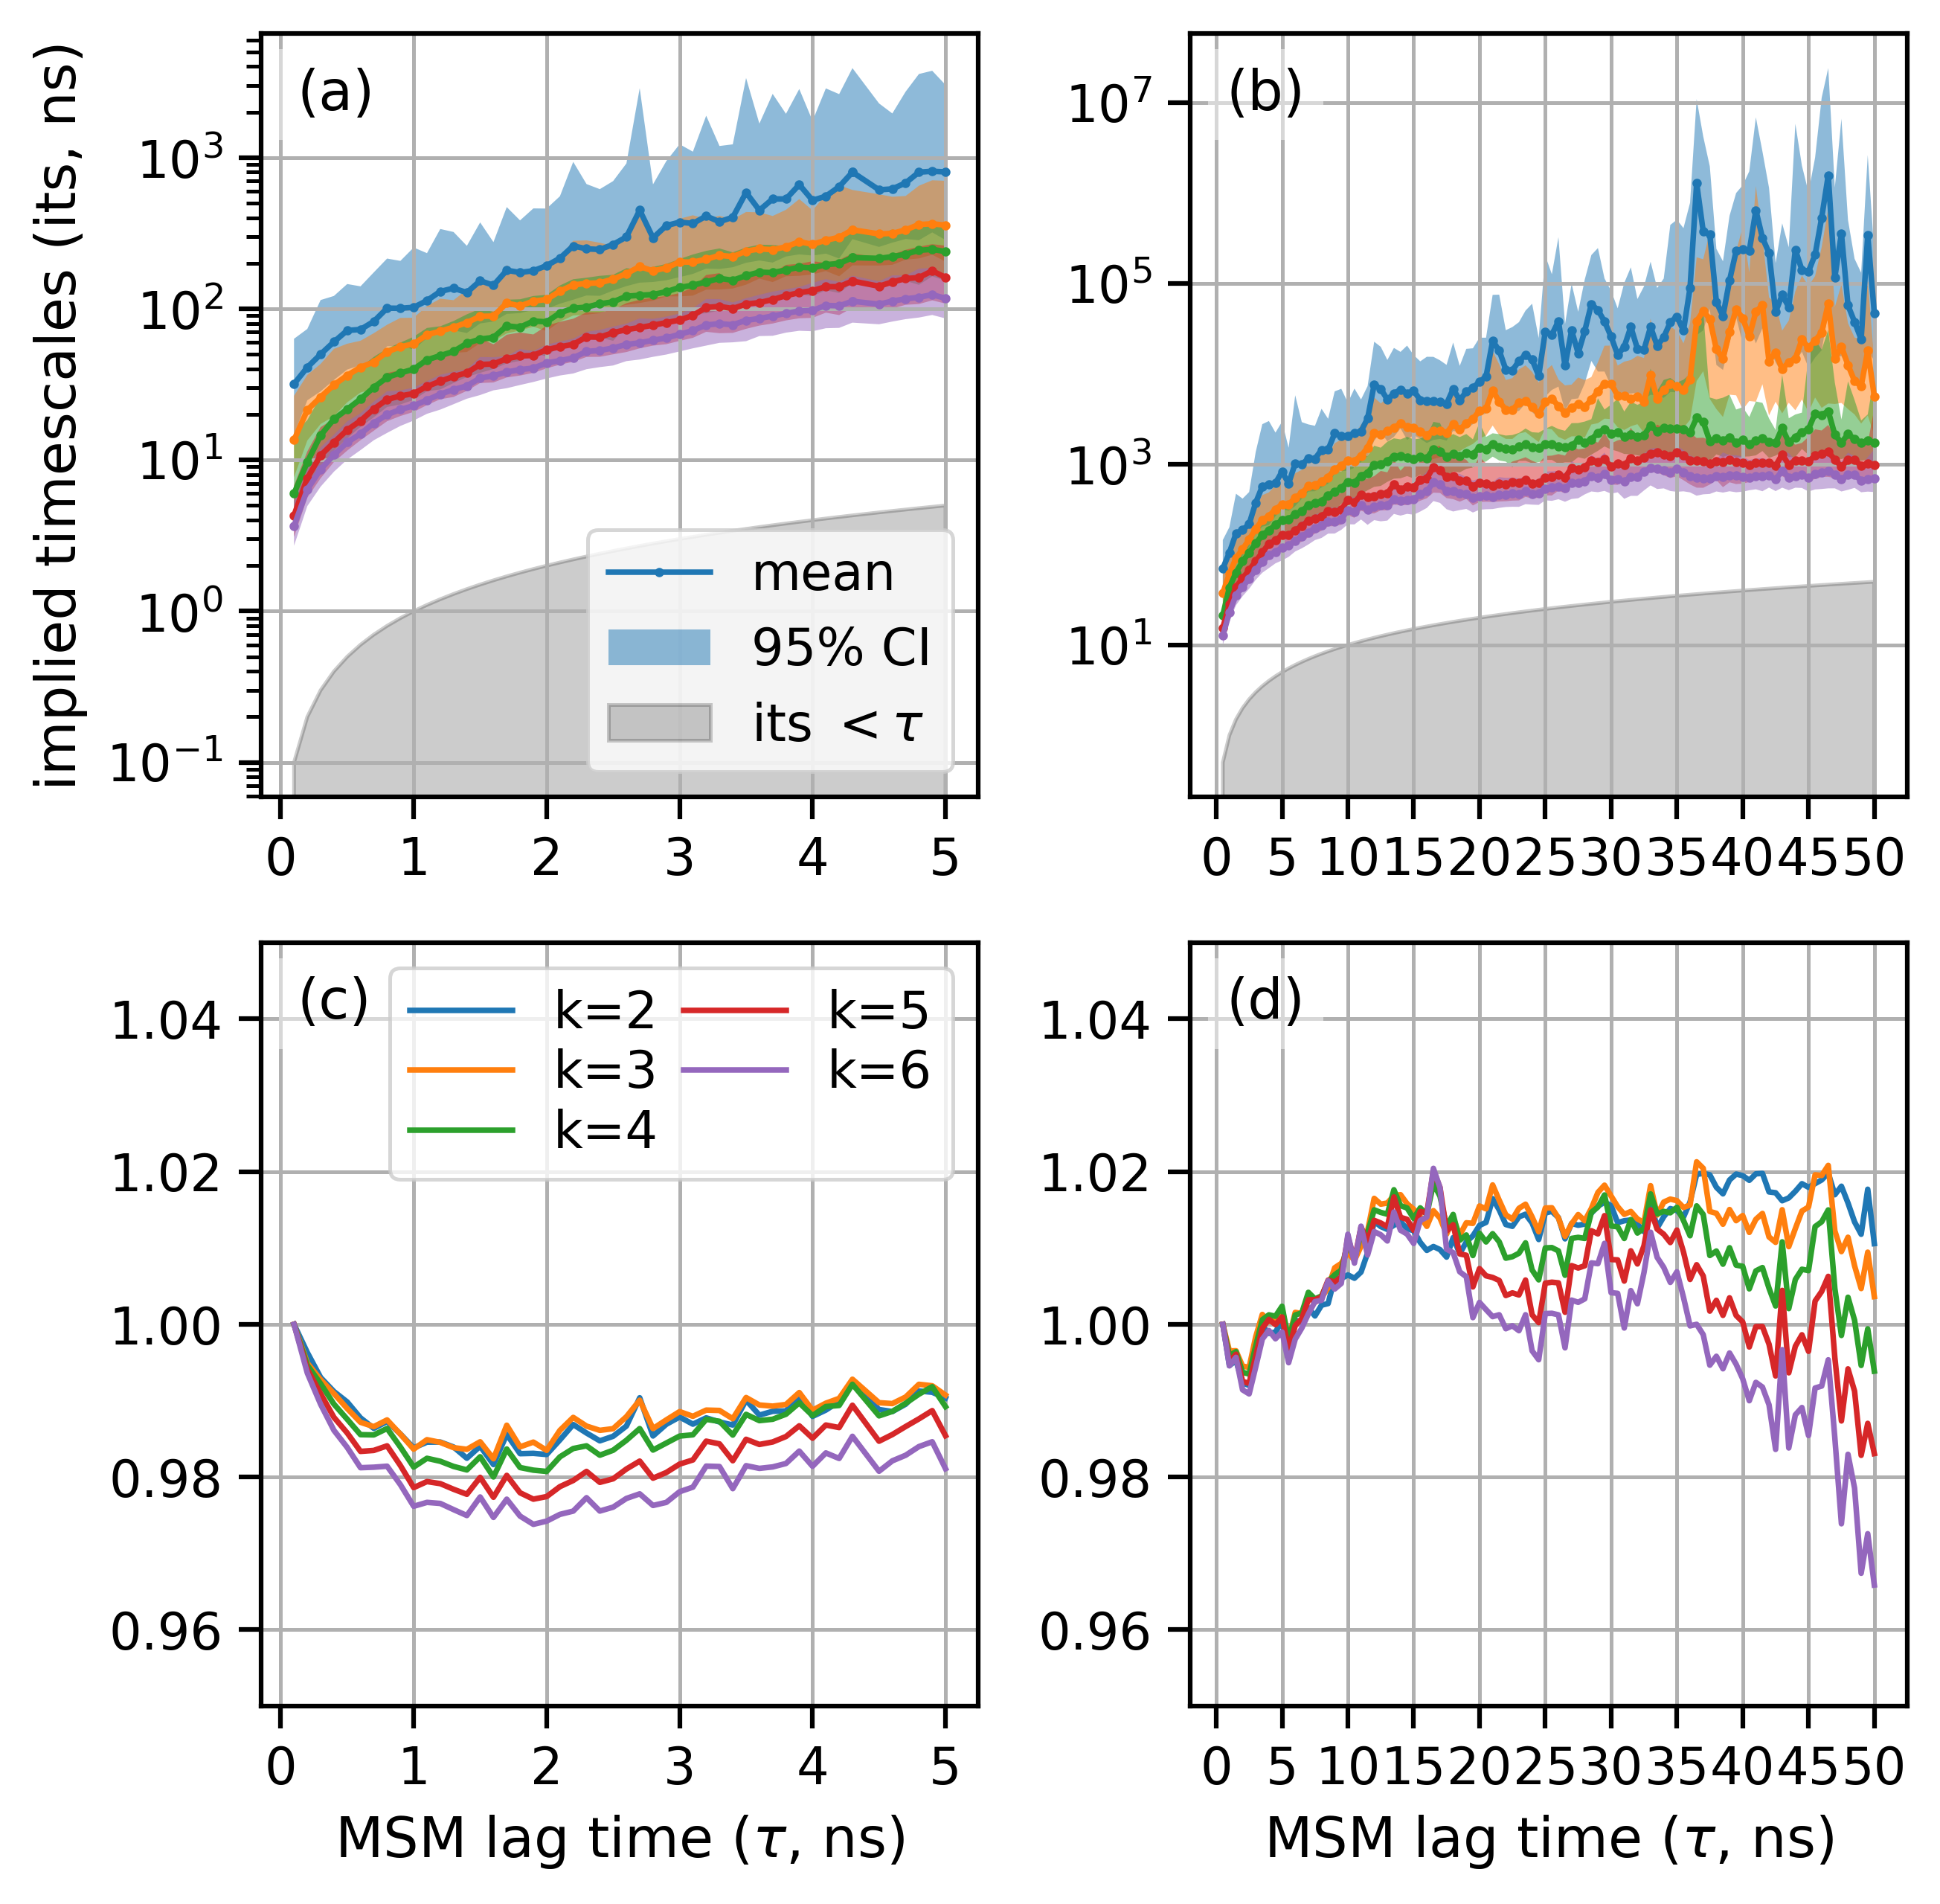
\includegraphics[width=0.8\textwidth]{chapters/aadh/figures/implied_timescales_D.png}
    \label{fig:its_d}
\end{figure}

A way out of this circular reasoning problem can be found by noting the following. First, the purpose of specifying the lag time and number of dominant processes is to provide a starting point from which the hyper-parameters of the MSM will be optimised. It is therefore only necessary that the choices do not affect the optimisation, rather than provide a strictly valid MSM specification. The lag time and number of dominant processes has only a small effect on the value of the VAMP-2 score as demonstrated by figure \ref{fig:its_d}. The first five implied timescales are shown a panel (a)  for $\SI{0}{\nano\second} < \tau(\mathrm{MSM}) < \SI{5}{\nano\second}$) and panel (b) for $\SI{0}{\nano\second} < \tau(\mathrm{MSM}) < \SI{50}{\nano\second}$. Underneath in panels (c) and (d) are shown the VAMP-2 scores with $k$ ranging from $2$ to $5$, which correspond to successively including the implied timescales shown in panels (a) and (b). The implied timescale (shown in blue) appears to become independent of the lag time from approximately \SI{10}{\nano\second}. However as panels (c) and (d) show the lag time has little effect on the VAMP-2 scores which vary by less than $\pm\SI{4}{\percent}$ from their initial values over all lag times. The value of $k$ also has little effect on VAMP-2 scores, at least up to $\tau(\mathrm{MSM})=\SI{15}{\nano\second}$ where their relative values start to diverge. Third, a  value of $\tau(\mathrm{MSM})$ and $k$ used for inference can be determined after optimisation through appropriate sensitivity analysis. A value of $\tau(\mathrm{MSM})=\SI{2}{\nano\second}$ was chosen based on the relatively small variation of the VAMP-2 score (panel (c) of figure \ref{fig:its_d}) and the larger number of observations that a small value affords. 

\begin{figure}
    \centering
    \mycaption{The ratio of successive implied timescales for a Markov state model with $\tau(\textrm{MSM})=\SI{2}{\nano\second}$, estimated using MCMC with $1000$ posterior samples. The blue dots and error bars are the mean and \SI{95}{\percent} credible intervals.}
    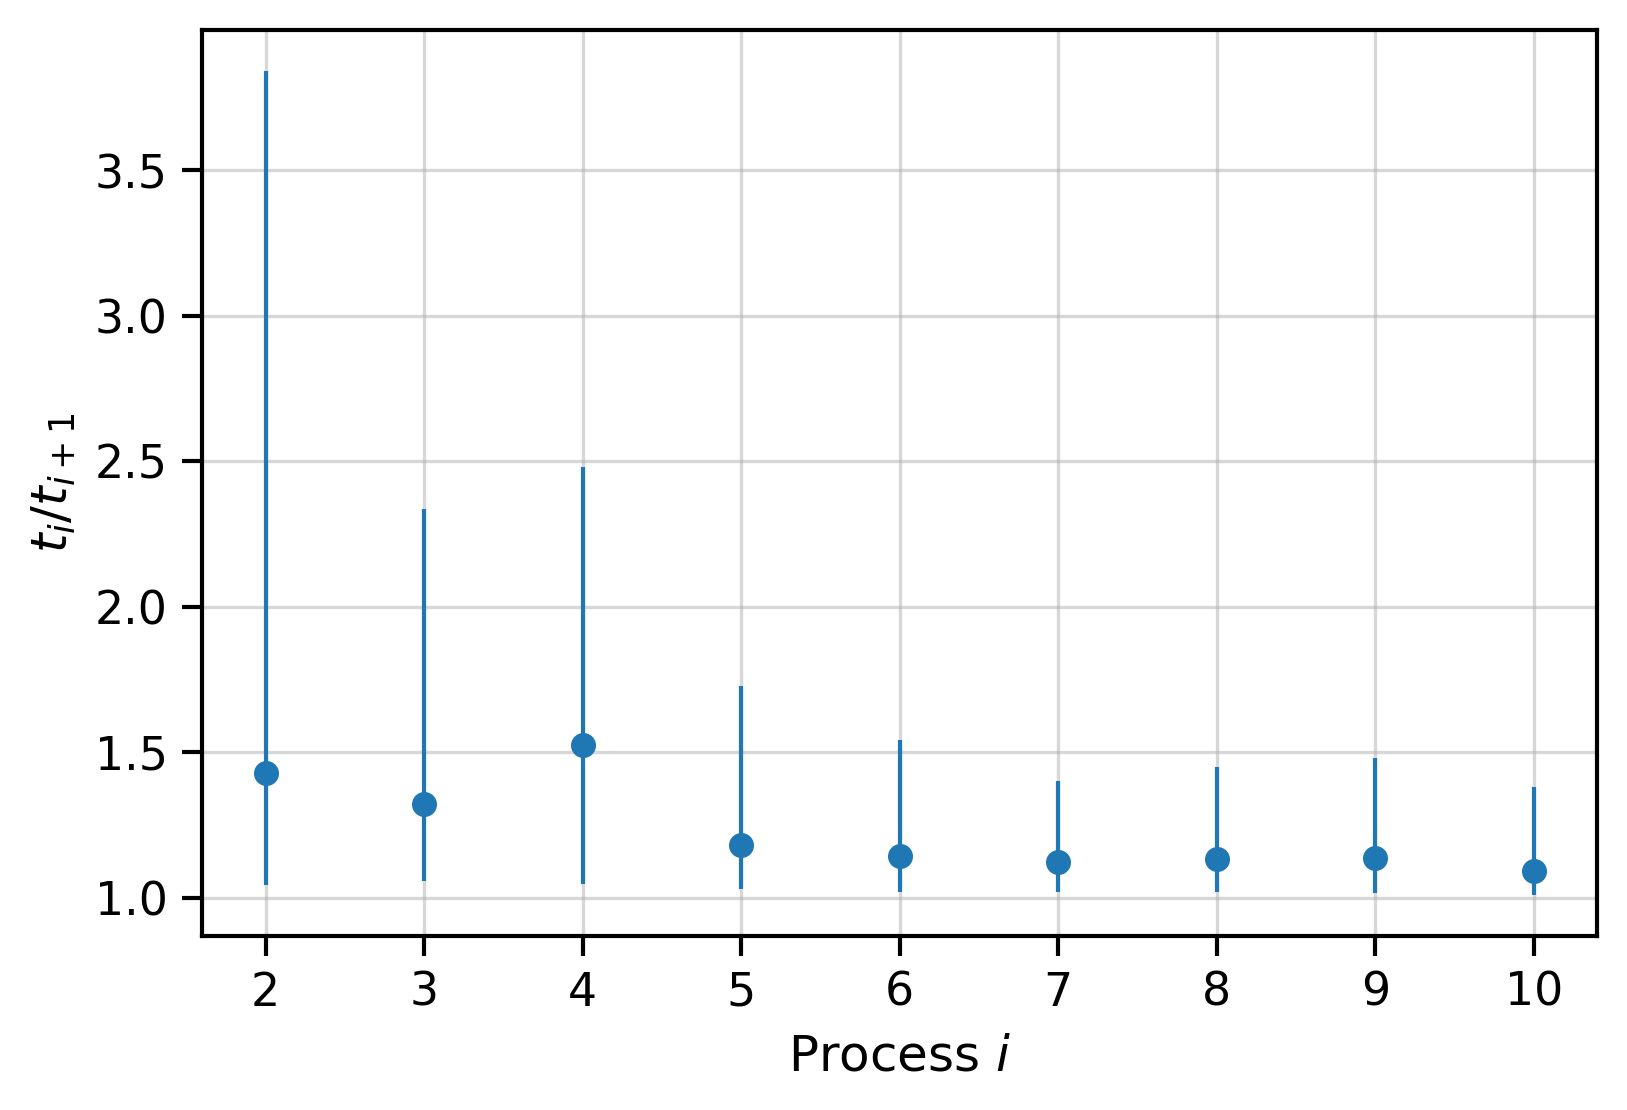
\includegraphics[width=0.8\textwidth]{chapters/aadh/figures/timescale_ratios_D.png}
    \label{fig:ts_ratios_d}
\end{figure}

The number of dominant processes was determined by inspection of the relative gaps in the eigenvalue spectrum at $\tau(\mathrm{MSM})=\SI{2}{\nano\second}$ shown in figure \ref{fig:ts_ratios_d}. The largest gap in the eigenvalues is between the fourth and fifth relaxation process. Therefore a value of $k=4$ was used. The issue of whether this is an appropriate value will be further investigated in the sensitivity analyses of chapter \ref{chap:msm} and in chapter \ref{chap:hmm} where the issue of the number of metastable states implied by a MSM will be addressed quantitatively. 

\section{Conclusions}
AADH is an important system for studying the effects of enzyme dynamics on catalysis due to the large kinetic isotope effect. Previous computational and experimental work determined the mechanism and estimated the free energy barriers using tryptamine as a substrate. The role of dynamics in explaining the temperature independent KIE in AADH is still unresolved. `Active dynamics` on the picosecond timescale have been suggested as facilitating tunneling, while  `passive dynamics', i.e. conformational dynamics, coupled with extensions of transition state theory, have also been suggested as explaining the behaviour of AADH's rate constant. To investigate the role of conformational dynamics in AADH, \SI{10}{\micro\second} of molecular dynamics simulations of the previously studied Schiff base intermediate were produced. A Markov lag time of $\tau=\SI{2}{\nano\second}$ and the number of dominant eigenvalues, $k=4$, were determined from an exploratory Markov state model. 

The validity of the simulations was limited however. An error in the preparation of the simulation resulted in the active site in the H chain missing an di-sulphide bond. The conformations of the H and D chains were radically different although surprisingly the H active site was more similar to the reactive conformations found in previous QM/MM studies. In addition, a number of unobserved residues were not modelled and there was correlation between each trajectory's initial configuration. Therefor a number of steps to improve this work: 

\begin{enumerate}
    \item Model the unobserved residues and fix the missing di-sulphide bonds in the crystal structure. 
    \item Solvate, energy minimize and equilibrate the initial structure. 
    \item From a long equilibration trajectory select $100$ configurations separated by \SI{10}{\nano\second} (the approximate Markov lag time from figure \ref{fig:its_d})), minimize and equilibrate these independently to create decorrelated initial configurations.
    \item  Use these initial configurations to seed $100$ production trajectories.
\end{enumerate}


\section{Appendix}

\begin{figure}[p]
    \centering
    \mycaption{LOW RESOLUTION! RMSD of the $\alpha$-Carbon atoms of AADH relative to the crystal structure. Each panel is a single trajectory, blue lines are the RMSD, black horizontal lines are the \SI{2.5}{\percent} and \SI{97.5}{\percent} quantiles (\SI{4.5}{\angstrom} and \SI{6.4}{\angstrom}, respectively) taken across all trajectories.}
    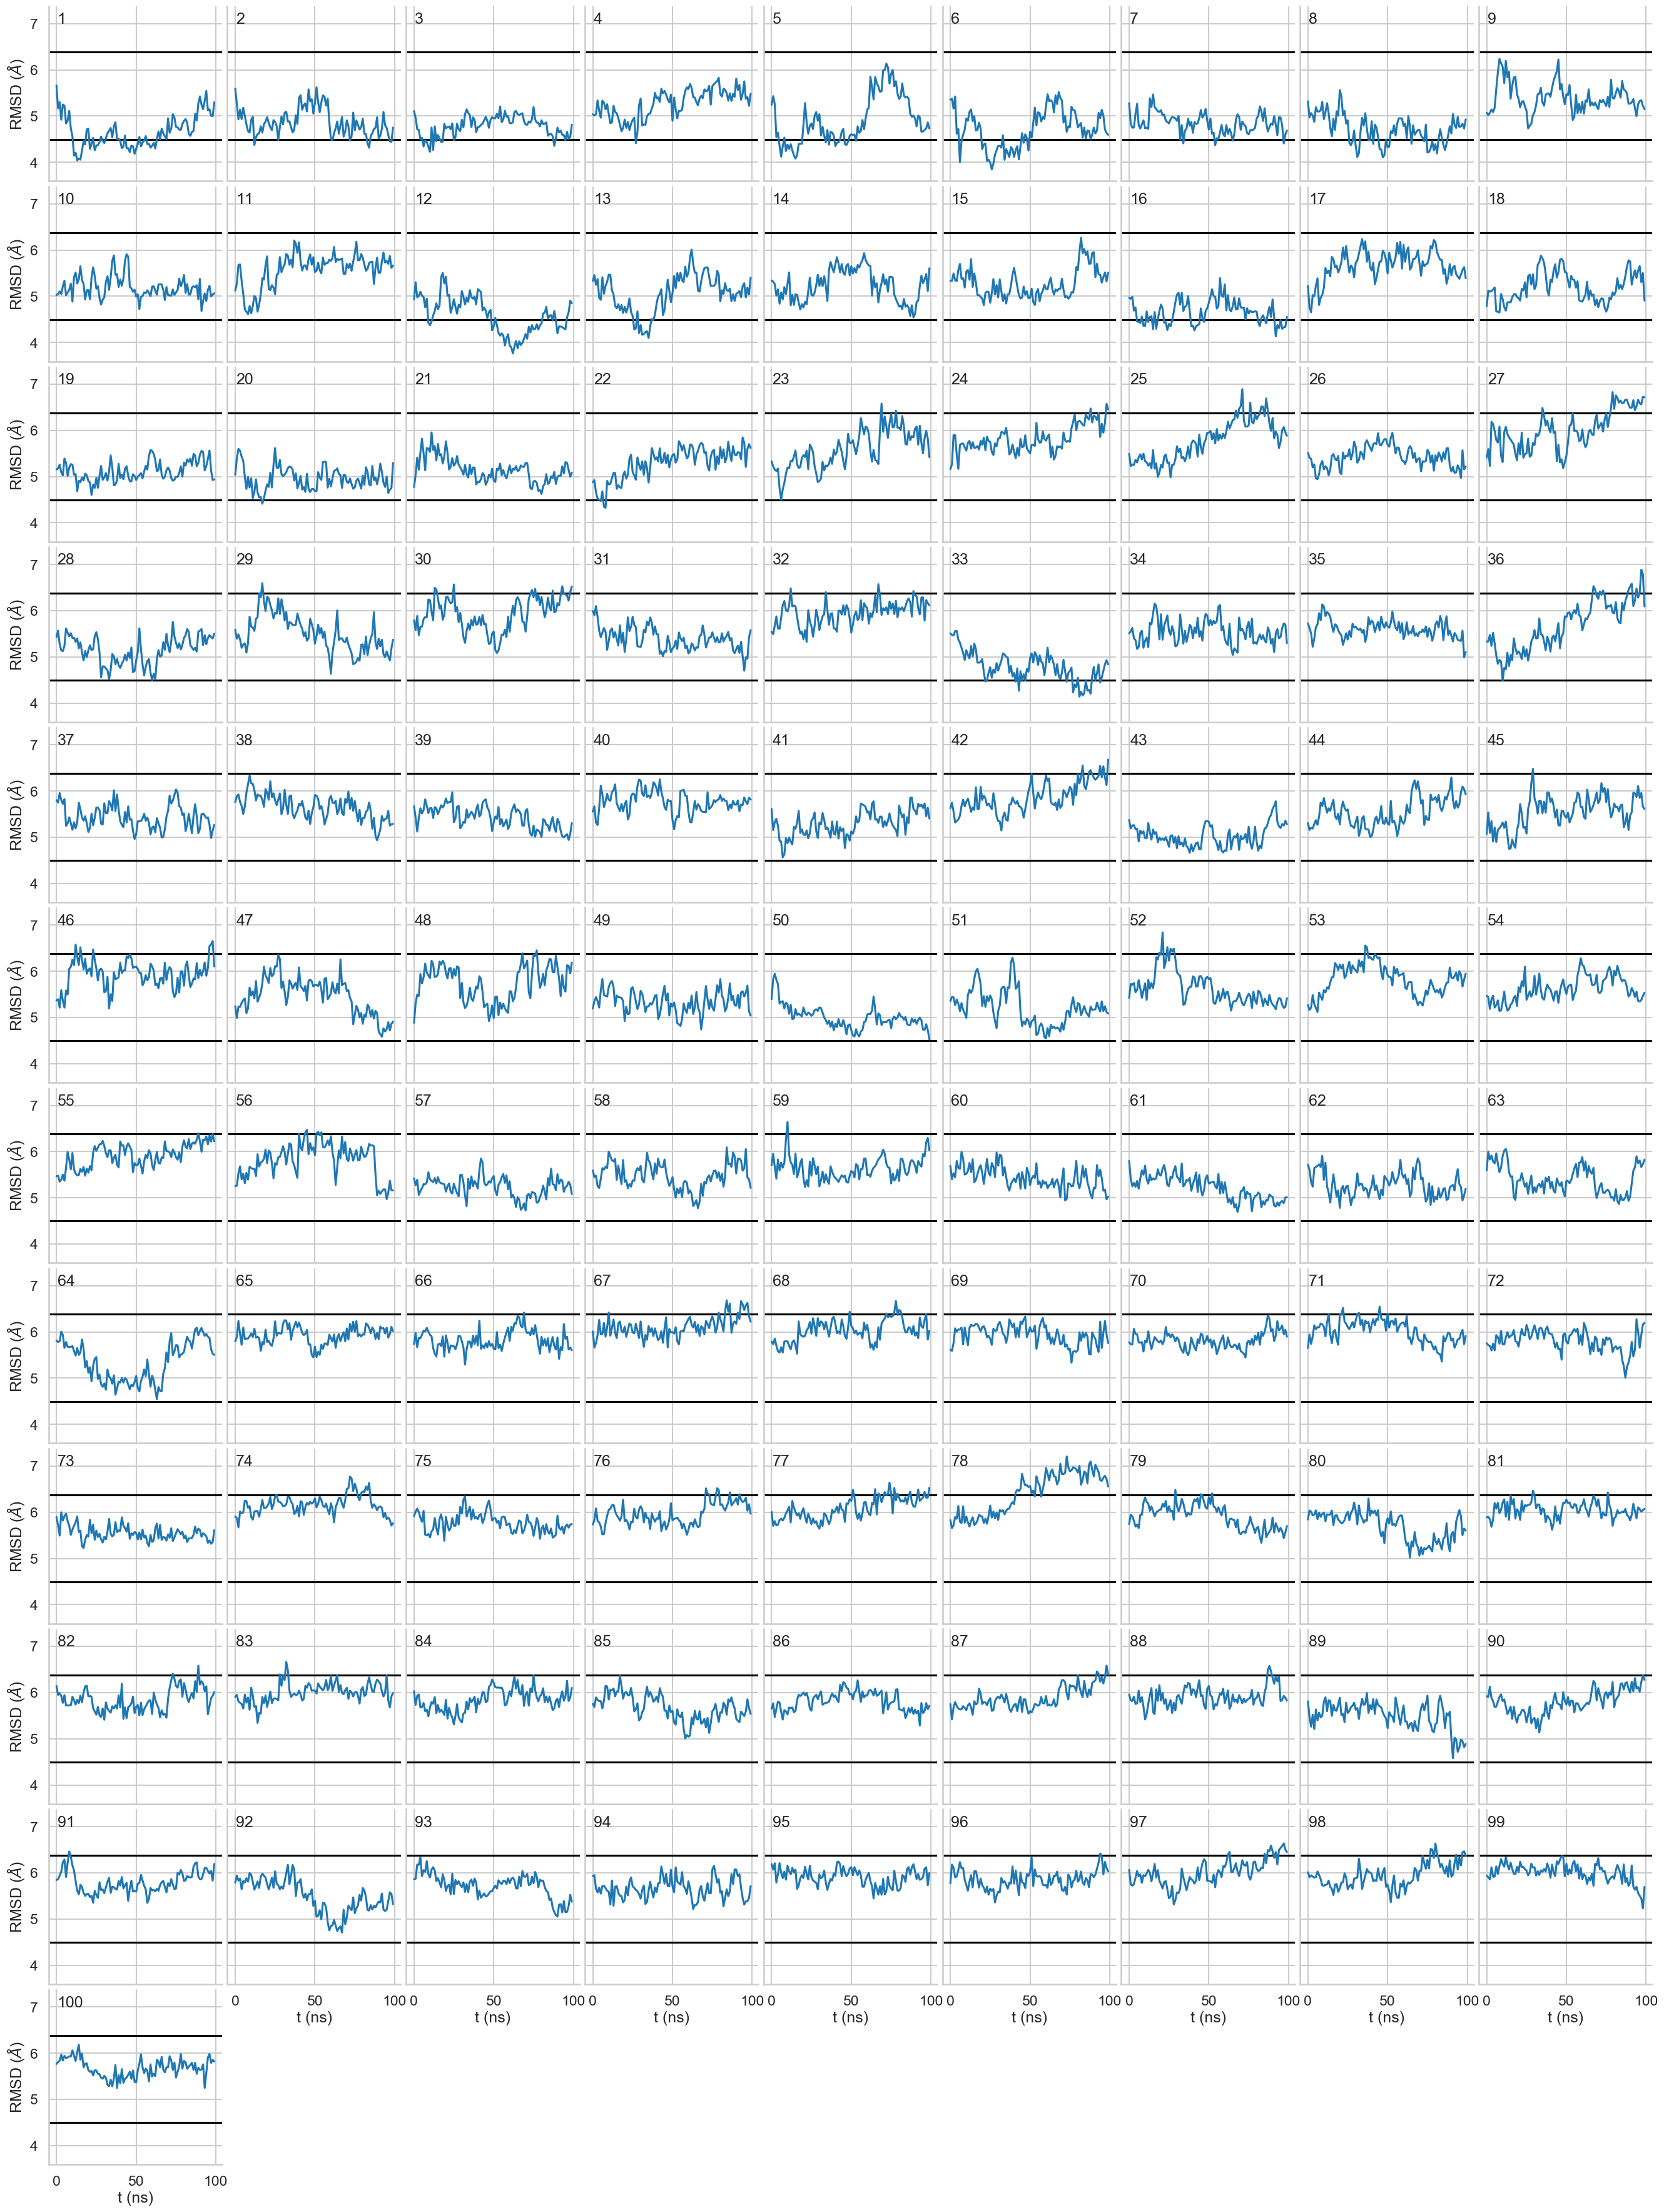
\includegraphics[width=0.9\textwidth]{chapters/aadh/figures/rmsd_backbone_ca.png}
    \label{fig:rmsd_ca}
\end{figure}

\begin{figure}
    \centering
    \mycaption{Secondary structure composition of trajectories $24, 27, 30, 42, 78, 87$ and $97$ as a function of time. The number of residues in each simplified secondary structure class \cite{kabschDictionaryProteinSecondary1983} are shown: `H' (green) refers to alpha helix, 3- and 5-helices; `E' (orange) refers to residues in beta-bridges or  beta ladder; `C' (blue) refers to turns, bends and all irregular elements.}
    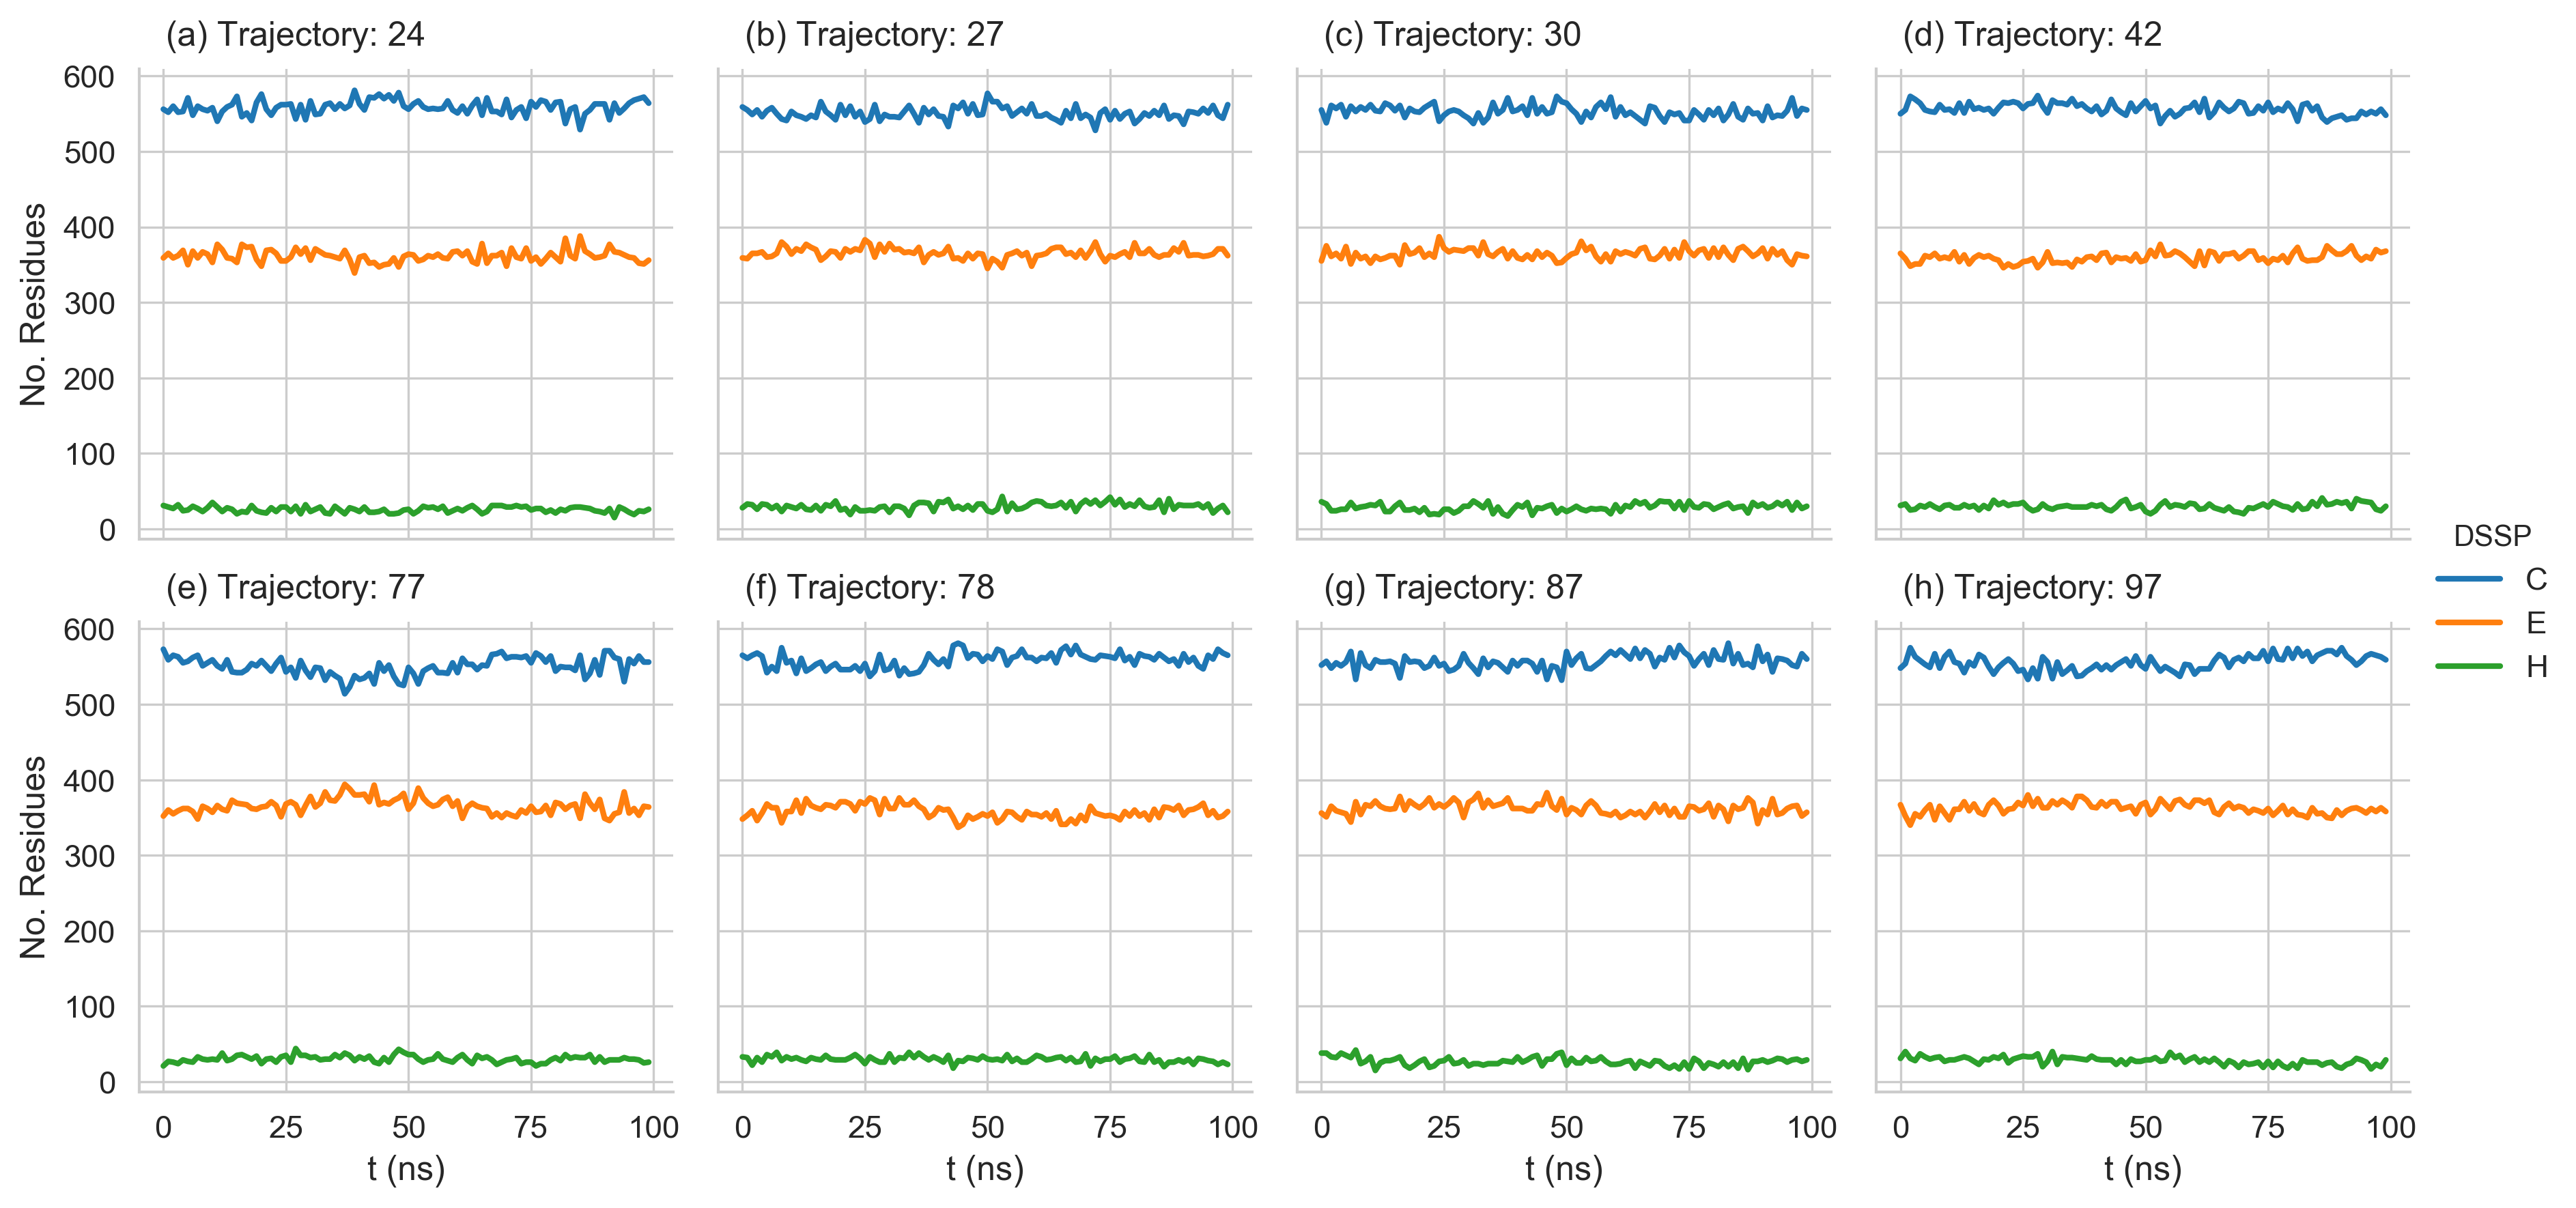
\includegraphics[width=0.9\textwidth]{chapters/aadh/figures/drift_trajs_dssp.png}
    \label{fig:dssp_trajs}
\end{figure}